% !TeX root = 0_build.tex
%
% 1
%
\section{Essential data skills}

	%
	%
  \newthought{This section shows how to manipulate datasets.} Start by opening the \ess:\\[1em]

		\begin{docspec}
			* Load the \ess, Rounds 4 (2008).\\
			use data/ess2008 if essround == 4 \& cntry == "FR", clear
    \end{docspec}
    
		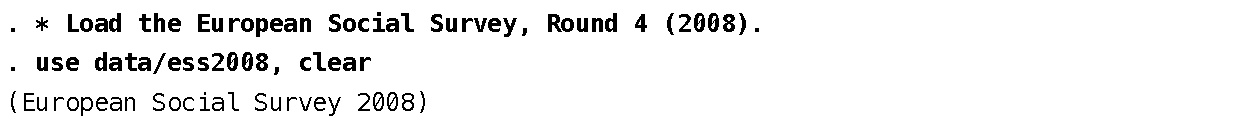
\includegraphics{use-ess}

  Notice that we are limiting the observations to a single country in a single survey round, as to get some data in the most basic cross-sectional structure. Similarly, when we use the \nhis, we limit the data to one year of data:%
  
    \begin{docspec}
      * Load the \nhis, latest survey year.
      use data/nhis9711 if year == 2011
    \end{docspec}
    
  You can build small-scale comparisons through time and space, \eg by comparing respondents from 2002 with respondents from 2012 in the \gss:%
  
    \begin{docspec}
      * Load the \gss, selected years.
      use data/gss0012 if inlist(year, 2002, 2012)
    \end{docspec}
    
  If you want to compare across countries from the \wvs or from the \ess, select a small number of cases out of the country code variables (consider three an operational maximum):%
  
    \begin{docspec}
      * Load data for one country (using numeric code).\\%
    	use data/wvs2000 if v2 == 4, clear\\[1em]%
      %
      * Load data for two countries (using names).\\%
      use data/wvs2000, clear\\%
      decode v2, gen(country)\\%
      keep if inlist(country, "Iran", "Iraq")\\%
      drop v2%
    \end{docspec}
    
	%
	%
	\newthought{Now take a look at the data.} Use the \cmd{browse} command to inspect the dataset in the Data Editor, which gives you a raw feel of the data in the `editor' layout that you know from spreadsheet editors:%

		\begin{docspec}
			browse
		\end{docspec}

  Optionally, you could have added a selection of variables to the \cmd{browse} command in order to show only some columns of the dataset:\\[1em]%

		\begin{docspec}
			use data/qog2013, clear\\
			browse ccode-version
      browse cname unna\_pop
		\end{docspec}

	The \cmd{browse} command is an exploratory command: it is a convenience tool to look at the data in read-only mode. You do not need to write exploratory commands like \cmd{browse} to your do-file, they are only meant to help you visualize the raw data.%
  	
  You should now be looking at the `top-left' observations and variables of the \QOG dataset, where you can see some unique identifier variables, like the version number of a dataset or the numeric codes and names of the country observations (Figure~\ref{fig:qog-browse}).%

		\begin{figure*}[h]
			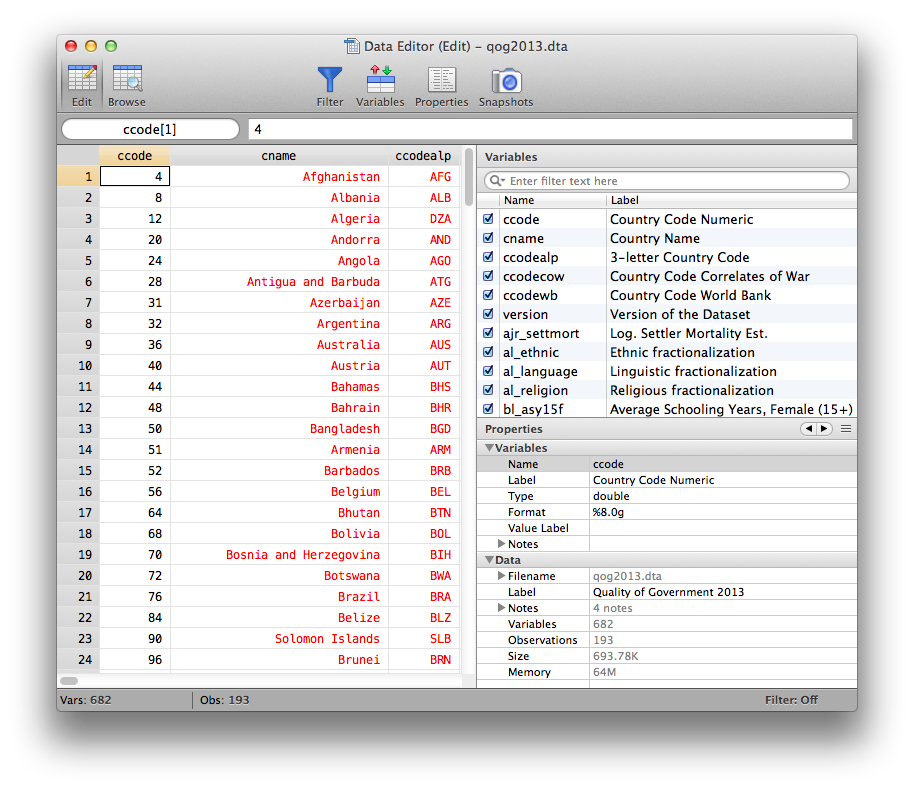
\includegraphics{qog-browse-screenshot}%
		  \caption{The Stata Data Browser, showing \QOG data.}%
		  \label{fig:qog-browse}%
		\end{figure*}

	%
	%
	Notice the different variable colors used in the Data Browser: in Figure~\ref{fig:qog-browse}, numeric measures are shown in black, whereas text descriptions, called `strings' in computer environments, are shown in red. While numeric values can be referred to directly in computing environments, strings require to be enclosed in \texttt{"quotes"} to be recognized as such.%
		
	There is another kind of variable \emph{encoding} that combines numeric values and text labels by assigning numbers to categories, groups or response items, like 1 coding for `Strongly agree' and 5 for `Strongly disagree'. These variables are shown in blue in the Data Browser, as illustrated with the \gss:\\[1em]%

		%
		\begin{figure*}[h]
			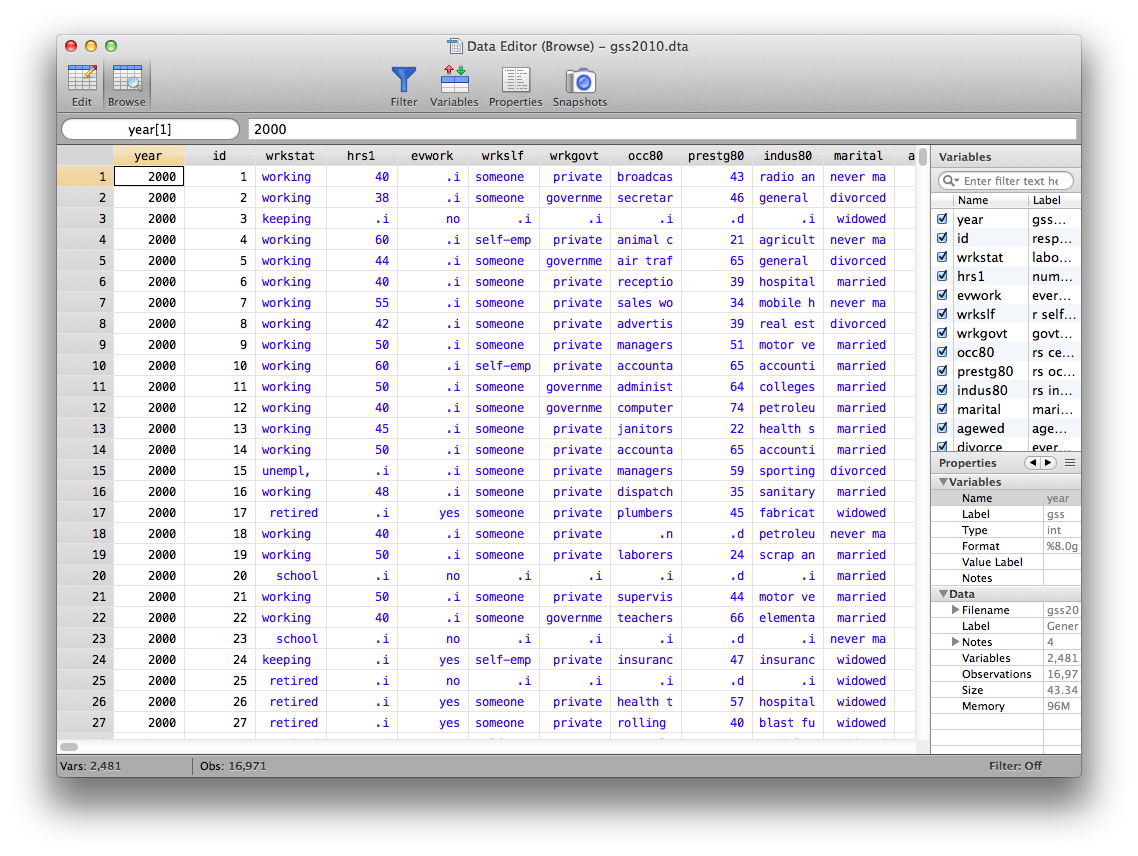
\includegraphics{gss-browse-screenshot}%
		  \caption{The Data Editor in Browse (read-only) mode, showing \GSS data.}%
		  \label{fig:gss-browse}%
		\end{figure*}

	In Figure~\ref{fig:gss-browse}, the blue color indicates that, for the \texttt{wrkstat} variable of the \gss, there is both a numeric coding scheme of the type 1, 2, etc., and a set of labels that correspond to employment categories: 1 for `Working full-time', 2 for `Working part-time', etc.%

	In Figures~\ref{fig:qog-browse} and \ref{fig:gss-browse}, some observations (rows of data) show values that start with a full period (\texttt{.}). This is how Stata codes \emph{missing values}. This scheme is idiosyncratic to Stata, and missing values can be coded differently (\eg by \texttt{NA}, \texttt{-1} or \texttt{999}) depending on the data collection protocol.%

	%
	%
	\newthought{Let's take a closer look at the values} by producing quick data extracts from a few variables and observations. We are going to use the \cmd[li]{list} command with the \cmd{li}{list} command followed by a few variable names and row numbers, from 1 to \texttt{\_N} where \texttt{\_N} is the total number of observations that you can get with the \cmd{count} command:%

		\begin{docspec}
			* Load Quality of Government data (2013).\\
			use data/qog2013, clear\\[1em]
	
			* Ask for the total number of observations.\\
			count\\[1em]
	
			* Alternately, ask for the "raw" result.\\
			di \_N
		\end{docspec}

		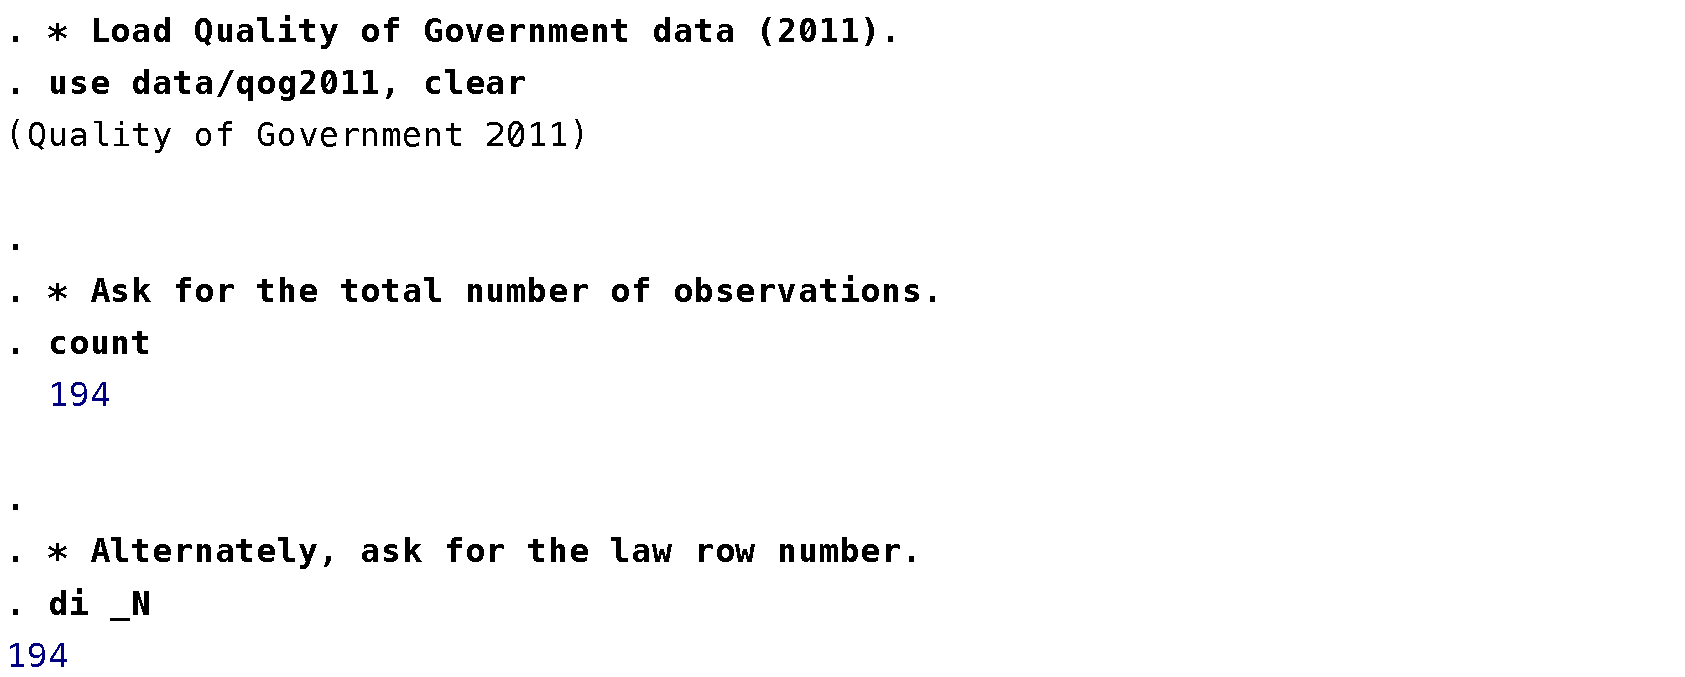
\includegraphics{qog-use-count}\\[1em]

  %%%

  \hlred{\textbf{Important:}} given its country-level unit of analysis, the \QOG dataset runs a smaller number of observations than the other teaching datasets used in the course. The largest possible sample of these countries is necessary to work with this dataset.%

  Thus, if you are using country-level data, do \emph{not} attempt to subset the \qog dataset to a particular selection of countries. The sample size is already very low in a country-level cross-section, as there are just that many countries at a given point in time.%
  
  If you still wish to take geographical context into account in your analysis, use the \cmd{kountry}\pkgfirst{kountry} package as described at p.~\pageref{qog:geo} to add regional descriptors to the \qog dataset, and compare across all available regions.%

  %%%
  
  \hlred{\textbf{Important:}} like the \cmd{browse} command, the \cmd[li]{list} command is just a convenience tool to take a look at the raw data. Listing the data is done only for exploratory motives: do not publish raw data listings or even save them to your log.%
  
  Similarly, when you are writing your analysis to a do-file, you do not need to make your code list the variables or the observations: describe only the parts of the data that are specifically relevant to your research, such as the names and labels of your selected variables.%

  %%%
  
  Let's use the \cmd{browse} command to read a few variables by passing their names to the \cmd{browse} command:%
		%
		\begin{docspec}
			browse cname-version\\
		\end{docspec}

%%%%%%%%%%fix!

\begin{docspec}
	* List first ten observations.\\
	li cname ccodealp in 1/10, clean\\[1em]
	
	* List last ten observations.\\
	li cname ccodealp in -10/l, clean
\end{docspec}

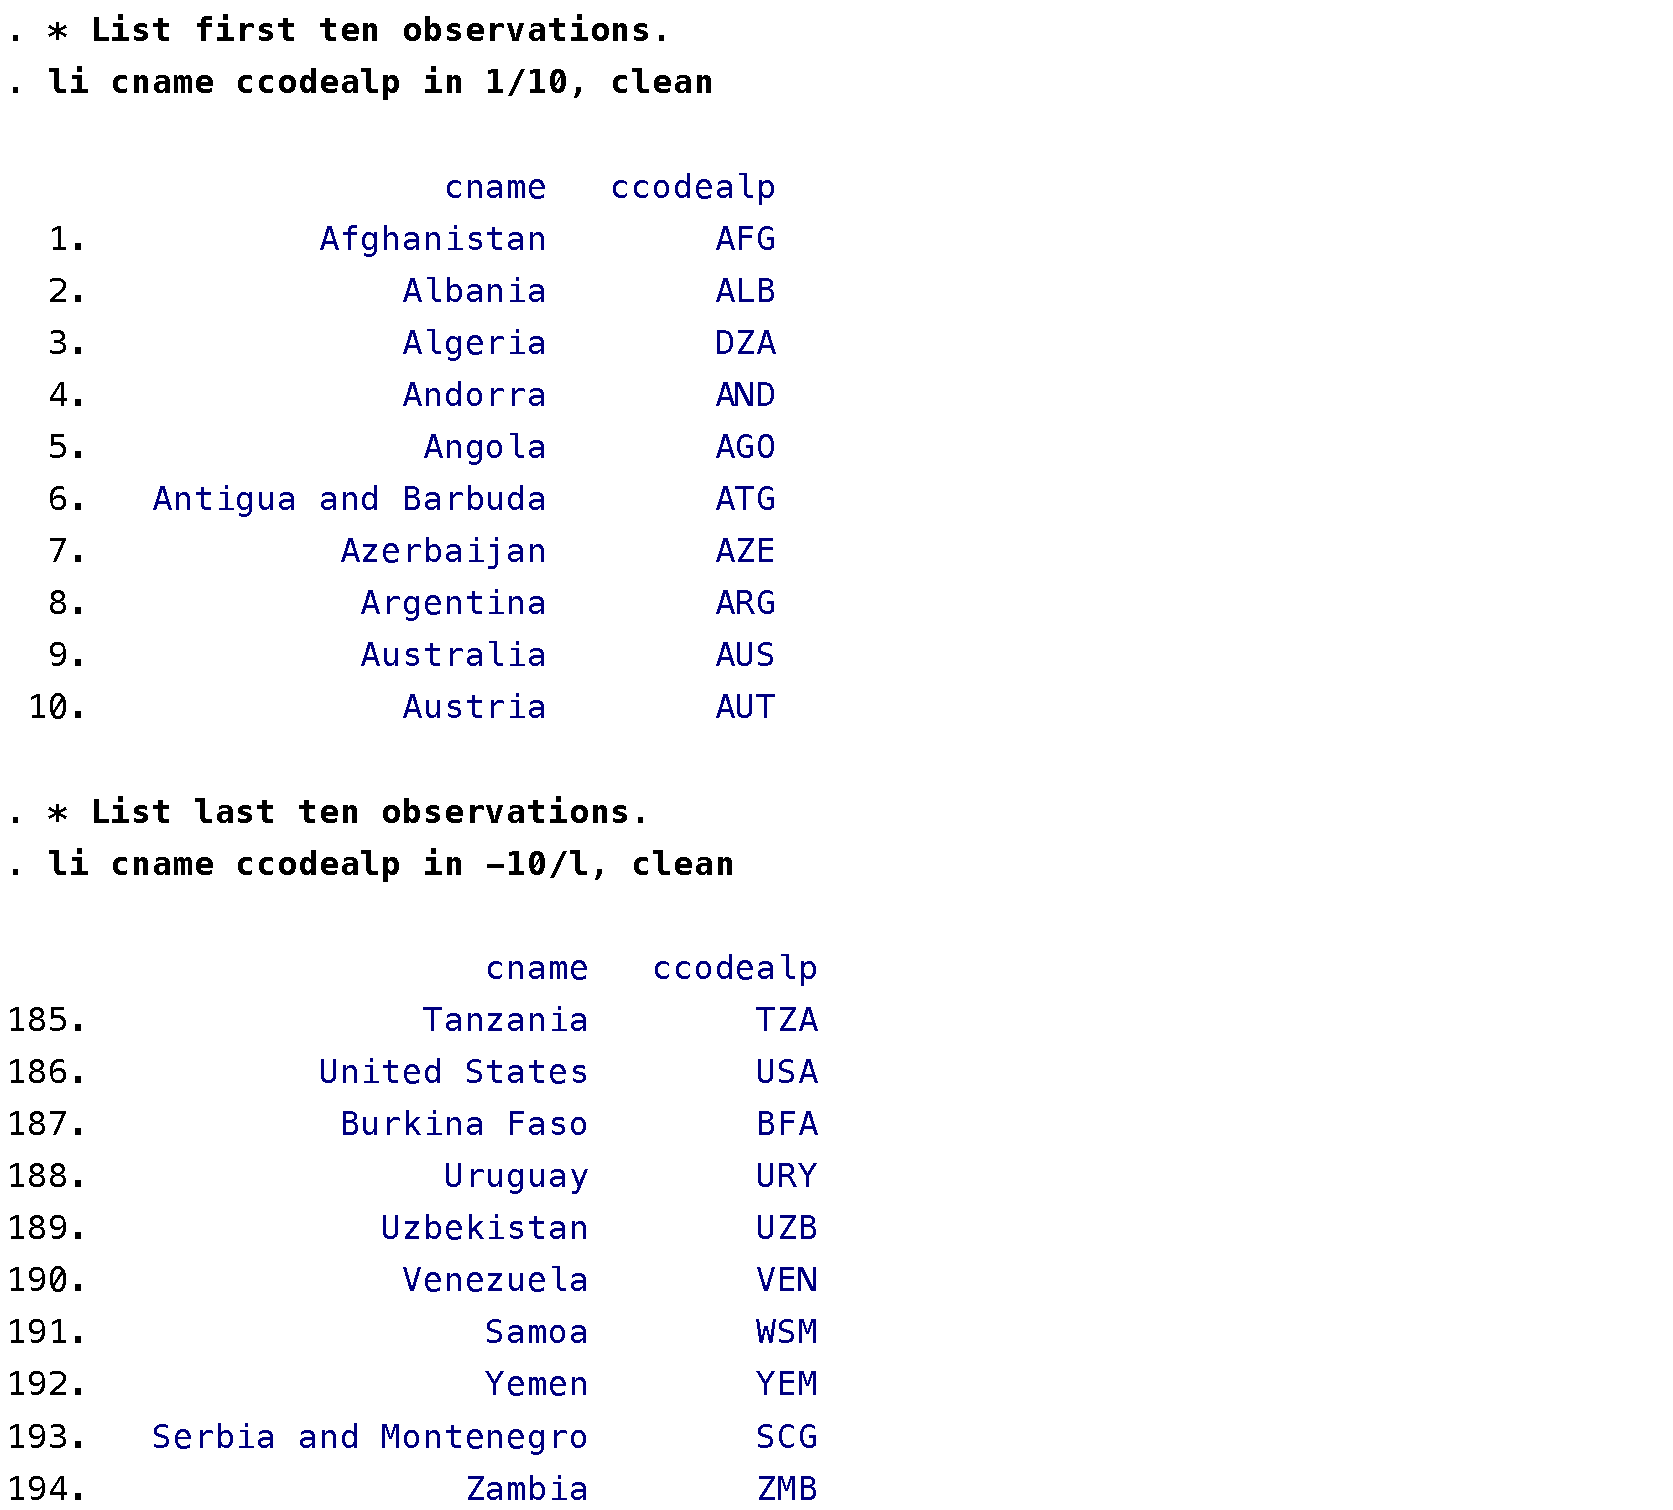
\includegraphics{qog-li-cname-ccodealp}\\[1em]

The \cmd{in} operator selects observations by their row number, which has limited use in most circumstances.%
	\index{Selectors!Observation ranges: \cmd{in}} %
	What you usually want to do instead is to select observations according to a given condition, which we will see how to do very soon.

\newthought{Describe the variables.} The command to list all variables in a dataset is \cmd[d]{describe}, which is more or less the first command that you want to run right after opening a dataset, if only to verify that the data have loaded properly. It can be used on its own or provided with a list of selected variable names:\\[1em]

\begin{docspec}
	use data/ess2008, clear\\
	d agea gndr edulvla
\end{docspec}

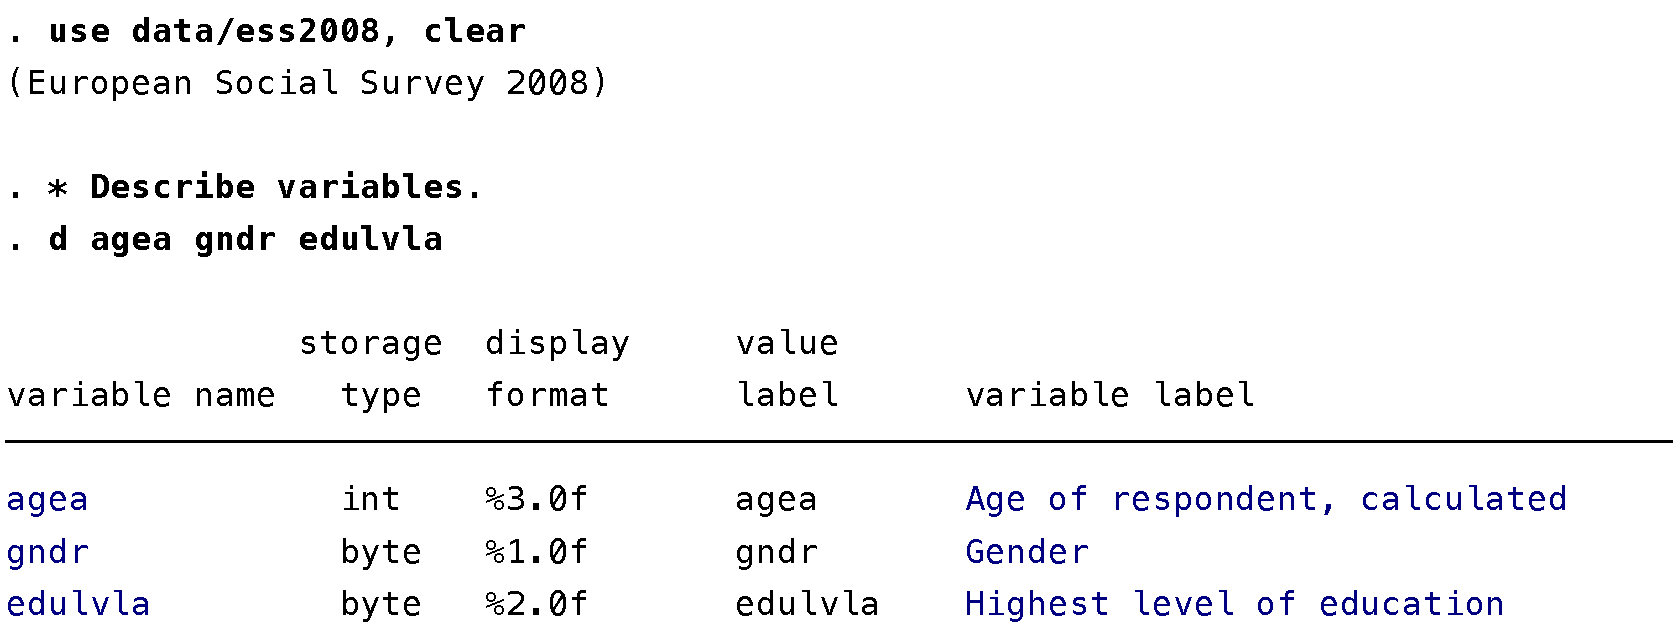
\includegraphics{ess-d}\\[1em]

To find variables by name or keyword, use the \cmd{lookfor} command:\footnote{You can also use the wonderful \cmd{lookfor\_all} command to search across datasets. Once installed by the course setup, the command allows you to search all datasets in the \data folder, as in this example with the \texttt{health} keyword:%
		%
		\begin{docspec}
			lookfor\_all health, dir(data)
		\end{docspec}}\\[1em]

\begin{docspec}
	use data/gss0012, clear\\
	lookfor homosex army
\end{docspec}

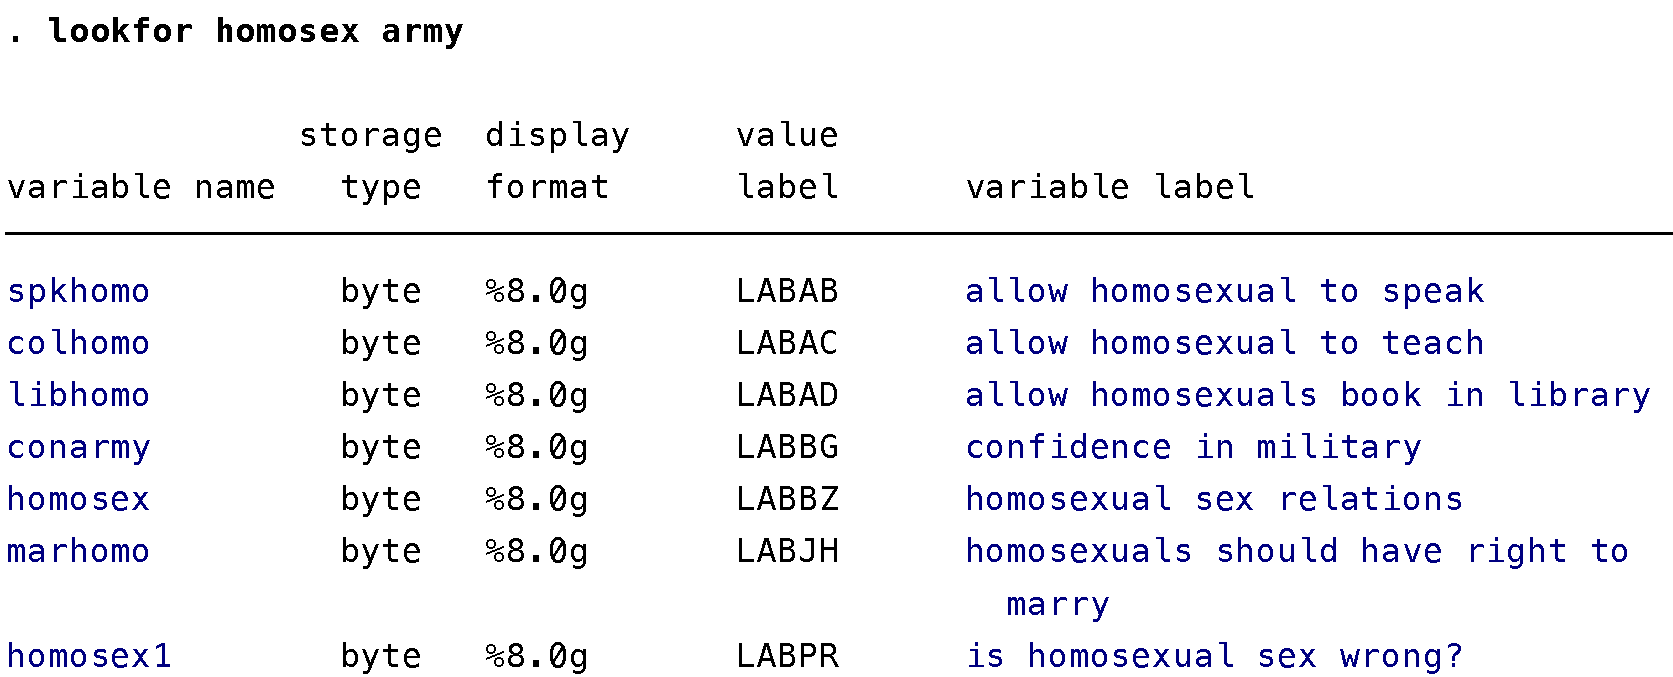
\includegraphics{gss-lookfor-homosex-army}\\[1em]

At that stage, in the best of cases, your variables of interest are ready for use, being present in the dataset in the format and with the descriptors that you want. An example would be this short selection of variables from the \QOG dataset:

	\begin{docspec}
		use data/qog2013, clear\\
		d cname ccodealp wdi\_fr wdi\_gdpc
	\end{docspec}
	
	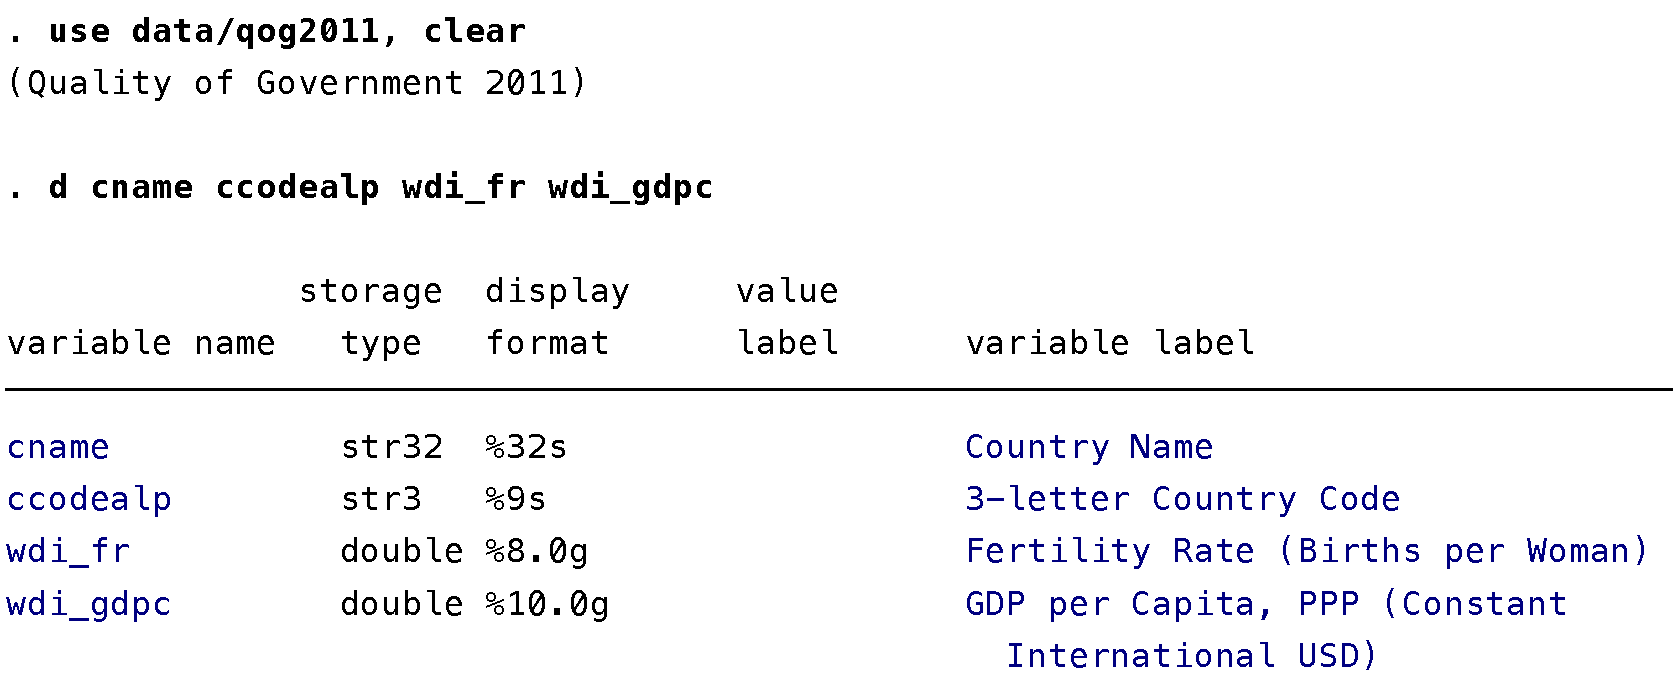
\includegraphics{qog-d}

Just two things might need a bit of adjustment at that stage. First, you might want to change the \emph{variable names} to more familiar ones by using the \cmd[ren]{rename} command. The command requires old and new variable names, and can work on many variables at the same time.%

For example, in the \qog dataset, you might want to pick your own name for the country name variable, which is often used during analysis:%

	\begin{docspec}
    * Rename country name variable.
    ren cname country
  \end{docspec}

  The \cmd[ren]{rename} command succeeds silently, with no output:

  %%fix: update
	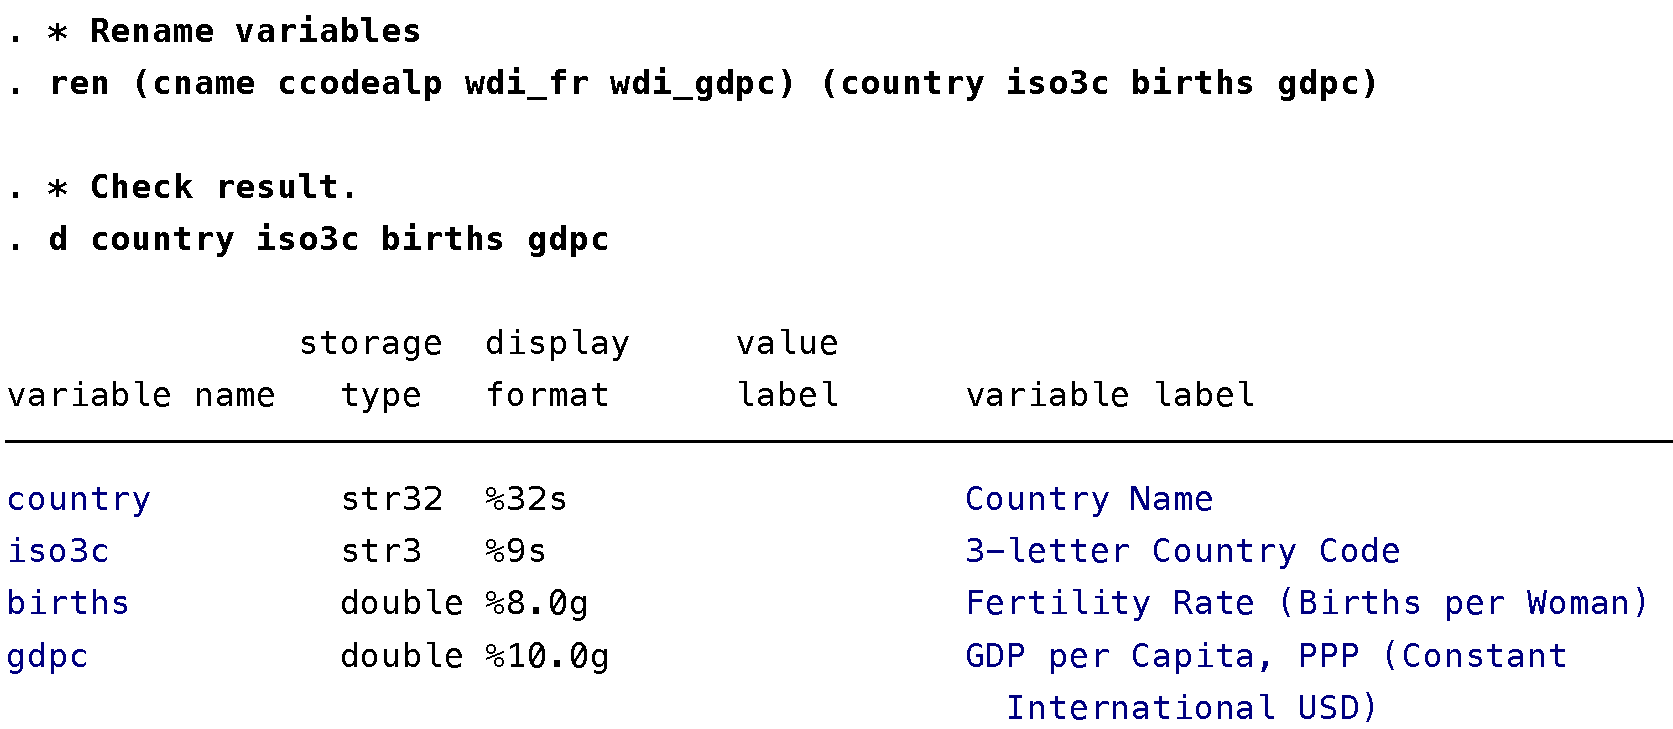
\includegraphics{qog-ren}

\label{qog:geo}%
Similarly, if you are interested in countries from a specific geographic region, you can obtain a simple continental from the \cmd{kountry} package, which creates a variable called \texttt{GEO} holding five UN~Stats standard regions.%
  \footnote{The \qog dataset includes the \texttt{ht\_region} variable holding ten regions.} %
  For consistency, we will rename the variable to lowercase:%

  	\begin{docspec}
      kountry ccode, from(iso3n) geo(un)\\
      ren GEO geo
    \end{docspec}

% Note: this variable can later be used to measure regional specificities, but it does \emph{not} come with an intrinsic reason for inclusion into your research design: it is still left to you to support the hypothesis of meaningful geographical effects in your data.%
  
You might also want to use the \cmd{renvars} \pkgfirst{renvars} command to batch rename variables (which is something that Stata~12 also knows how to do, with more code). Use a backslash to separate the list of old and new variable names:%

	\begin{docspec}
    * Rename two WDI indicators.
    renvars wdi\_fr wdi\_gdpc \textbackslash{} births gdpc
		* Check result.\\
		d country births gdpc
	\end{docspec}

\index{Variables!Labels}\index{Labels!For variables}%
Then, you might also want to adjust \emph{variable labels}, which are the short pieces of text attached to each variable. Use the \cmd[la var]{label variable} command to change the variable label to something meaningful, \eg mentioning the unit of measurement of the variable.%

\begin{mybox}
  \paragraph{Example: political positioning (\ESS)}%
    \label{ess:lrscale}%
  %
  The \texttt{lrscale} variable of the \ess is an 11-point self-placement scale measure of political position, from left-wing (\texttt{0}) to right-wing (\texttt{10}):%
  
	\begin{docspec}
		use data/ess0810, clear\\
    codebook lrscale, c
  \end{docspec}

  To remember that coding, we can rename the variable to the mnemonic \texttt{rightwing}, as to imply that the higher the value of the variable is, the more right-wing the respondent declared to be:%
  
	\begin{docspec}  
		ren lrscale rightwing
		la var rightwing "Left-wing to right-wing (0-10)"\\
  \end{docspec}

  The label makes certain that the coding will be unambiguous to the reader in the future. Relabelling the variable to indicate how the measure is to be interpreted is also useful to later include the variable in a descriptive table.%
  
	\begin{docspec}
    d rightwing
	\end{docspec}

\end{mybox}

It is generally a good idea to have variable labels that will provide something informative to graphs where they appear as axis titles. Short titles with some indication of the underlying coding scheme usually do the trick.

One last aspect of data preparation that might be of some use is to subset (\ie to restrict) the dataset to the variables that you are going to use. To do so, pass the names of your variables to the \cmd{keep} option, as in \statacode{keep v1 v2 v3} etc. I however strongly suspect this requirement to be some form of older computing age legacy that would now apply only in only few cases of large data and small memory, so I recommend \emph{not} doing this by default.

\newthought{Essential data skills} include being able to further distinguish between types of variables (p.~\pageref{sec:variable-types}), to encode missing values so that the software recognizes them (p.~\pageref{sec:missing-values}), and to recode variables to alternative groups and categories (p.~\pageref{sec:categorical-recodes}).

These skills are explained below, along additional skills that will be useful to those working with external data sources, and more advanced skills for more complex research projects.%

%
% 1.1
%
\subsection{Variable types}
\label{sec:variable-types}

You will usually want to know two things about all your variables:

\begin{enumerate}
	\item What is the \textbf{unit of measurement} of the variable? Is it meaningful, or are the numbers just a convenient to order or code some category?
	
Note in passing that what you see in a dataset is the endpoint of a social activity, and that data of all sorts are hardly neutral assets. Quantification and commensuration are conflictual process that can have critical policy implications, especially in the case of rankings and benchmark indicators of public and private performance.%\cite{EspelandStevens:2009n,Briatte:2012a,DavisFisher:2012x}

	\item What is the \textbf{coding scheme} to read the values? Is the variable made of strictly text, strictly numbers, or does it use both jointly?
\end{enumerate}

Variables can be classified into a certain number of types from these criteria: if the unit of measurement includes a true zero, if the measures can be meaningfully ordered, whether they are equally intervalled, …

But then, you probably want to learn only about the three practical categories to which all variables types eventually boil down when it is time to actually get to manipulate the data:

\begin{enumerate}
	\item \textbf{Continuous variables} like age, income, GDP per capita, male-to-female income ratio, percentage of people below the poverty line…
	\item \textbf{Categorical variables} like age and race \emph{groups}, income \emph{deciles} or \emph{bands}, marital status, 5-point agreement scales…
	\item \textbf{Dummy variables} (`dummies') that take only 0 and 1 values to code for a TRUE/FALSE statement like `is married' or `is a democracy'.
\end{enumerate}

\begin{description}
	\index{Variables!Continuous variables}%
	\item[Continuous variables] have meaningful units and generally high dimensionality: they take many different numeric values that require a unit of measurement, like years or constant dollars, to be interpreted. The average value of a continuous variable can be meaningfully interpreted: `the average fertility rate' is meaningful to some extent, while `the average race' is meaningless.

	Continuous variables are called `continuous' because their values can be any number in a given segment of the real number line $\mathcal{R}$. For many variables like age or GDP growth, there is an infinity of values: your exact age can be any positive number $(26, 26.1, 26.01, ...)$, and GDP growth theoretically ranges from negative to positive infinity. The effective number of values taken by a continuous variable is limited by measurement precision and by the empirical range of the variable: age, for instance, is usually a variable composed of around 100 possible values expressed in years.

	The example below shows the output of the \cmd{codebook} command for a continuous variable from the \qog dataset. The \texttt{wdi\_gdpc} variable measuring GDP per capita takes 178 unique values, ranging from 226 to over 63,000 constant international dollars:\\[1em]
	
	\begin{docspec}
		use data/qog2011, clear\\
		codebook wdi\_gdpc
	\end{docspec}
	
	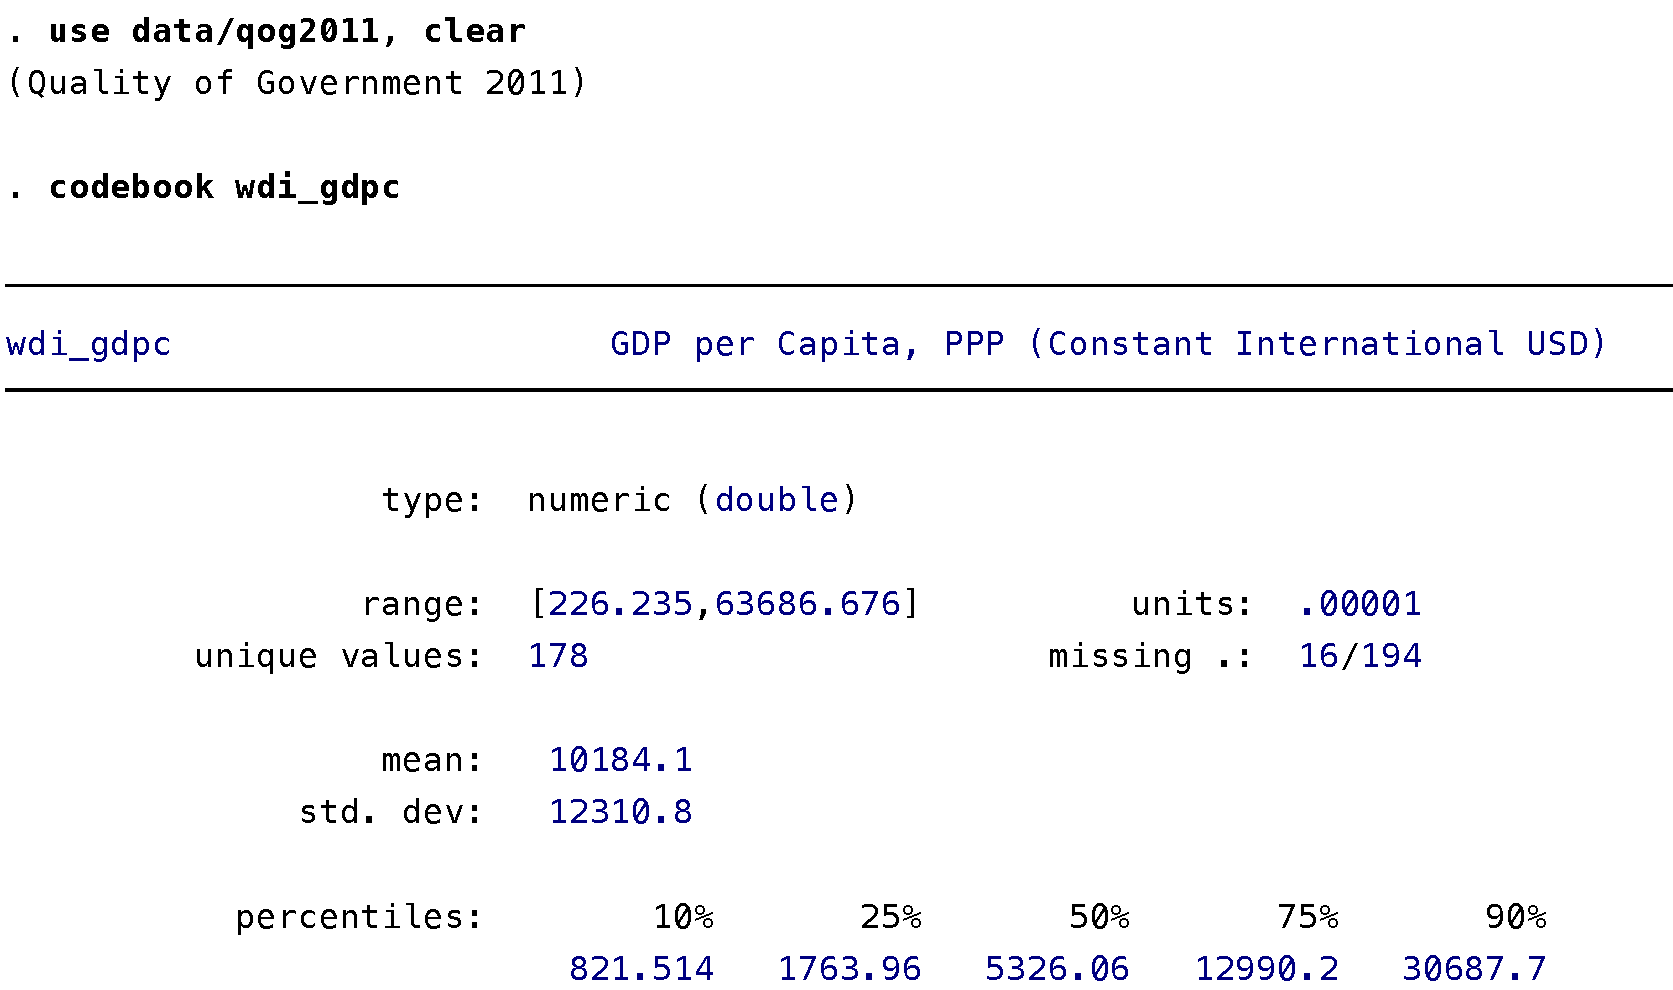
\includegraphics{qog-codebook-gdpc}\\[1em]
	
	We can now use the \cmd[su]{summarize} command to get the average height (measured in inches) and weight (measured in pounds) of U.S. residents over the past decade or so:
	
	\begin{docspec}
		use data/nhis9711, clear\\
		su weight height
	\end{docspec}
		
	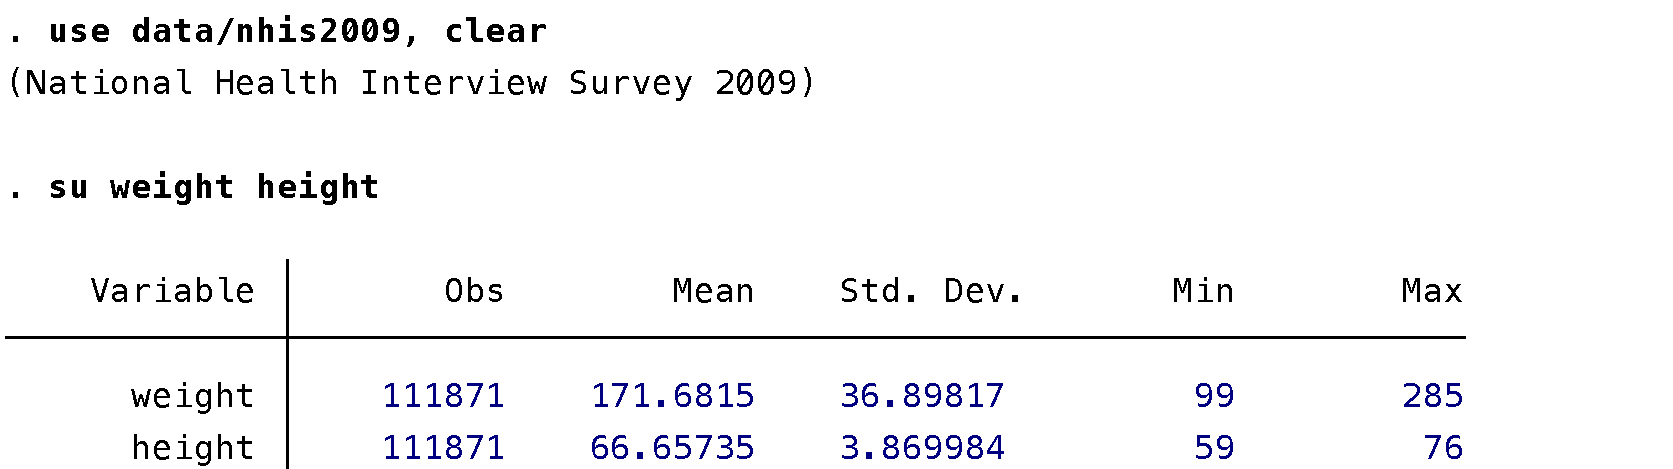
\includegraphics{nhis-su-height-weight}\\[1em]
	
	Using that combination of variables, we can generate the Body Mass Index of the sample population from its inch/pound equation. We then label the variable with an informative label and finally summarize the new variable with the \cmd[su]{summarize} command:\\[1em]
	
	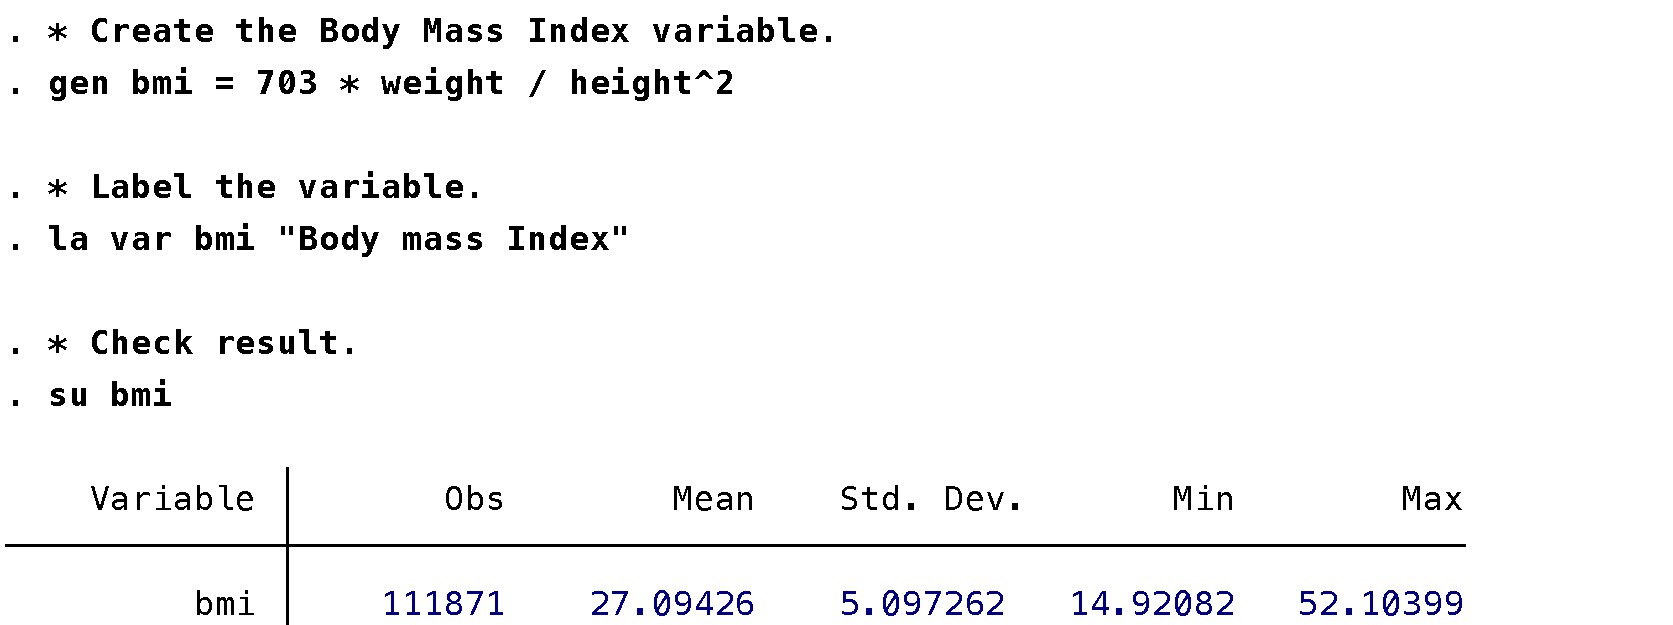
\includegraphics{nhis-gen-su-bmi}\\[1em]
	
	Using the \cmd[gen]{generate} and \cmd[su]{summarize} commands is probably the simplest routine to create and summarize a continuous variable. There are cases, however, where other commands are better tools for recoding a variable to a new one.
	
	\index{Variables!Categorical variables}%
	\item[Categorical variables] are artifical numeric codes for discrete entities that can be either ordered, like a 4-point scale of agreement to a question that goes from 1 `Strongly agree' to 4 `Strongly disagree', or unordered, like ethnicity, religious denomination, race or any other nominal marker for which there is no true ordering. These variables do not have meaningful averages but usually come with \emph{text labels} to describe each category: 1 will code for `Married', 2 for `Single', 3 for `Widowed', etc.

	A categorical variable might correspond to a continuous variable at lesser dimensionality: age groups, for example, are a recode of age measured in years into a handful of ordered categories (15-24, 25-34, etc.), which allow to speak in aggregates like `the youth', `the workforce' or `seniors'. In such \emph{ordinal} variables, the \emph{cutoff points} are expected to follow some kind of numeric convention: age groups might be coded per decade, income might be coded by decile or by bands of thousands of constant dollars, and so on.

	The example below shows the output of the \cmd{fre} command for a categorical variable from the \ess dataset.\pkgfirst{fre} Household net income, which was originally measured in country-specific units, was aggregated to deciles for cross-country comparability:\\[1em]

	\begin{docspec}
		use data/ess2008, clear\\
		fre hinctnta
	\end{docspec}

	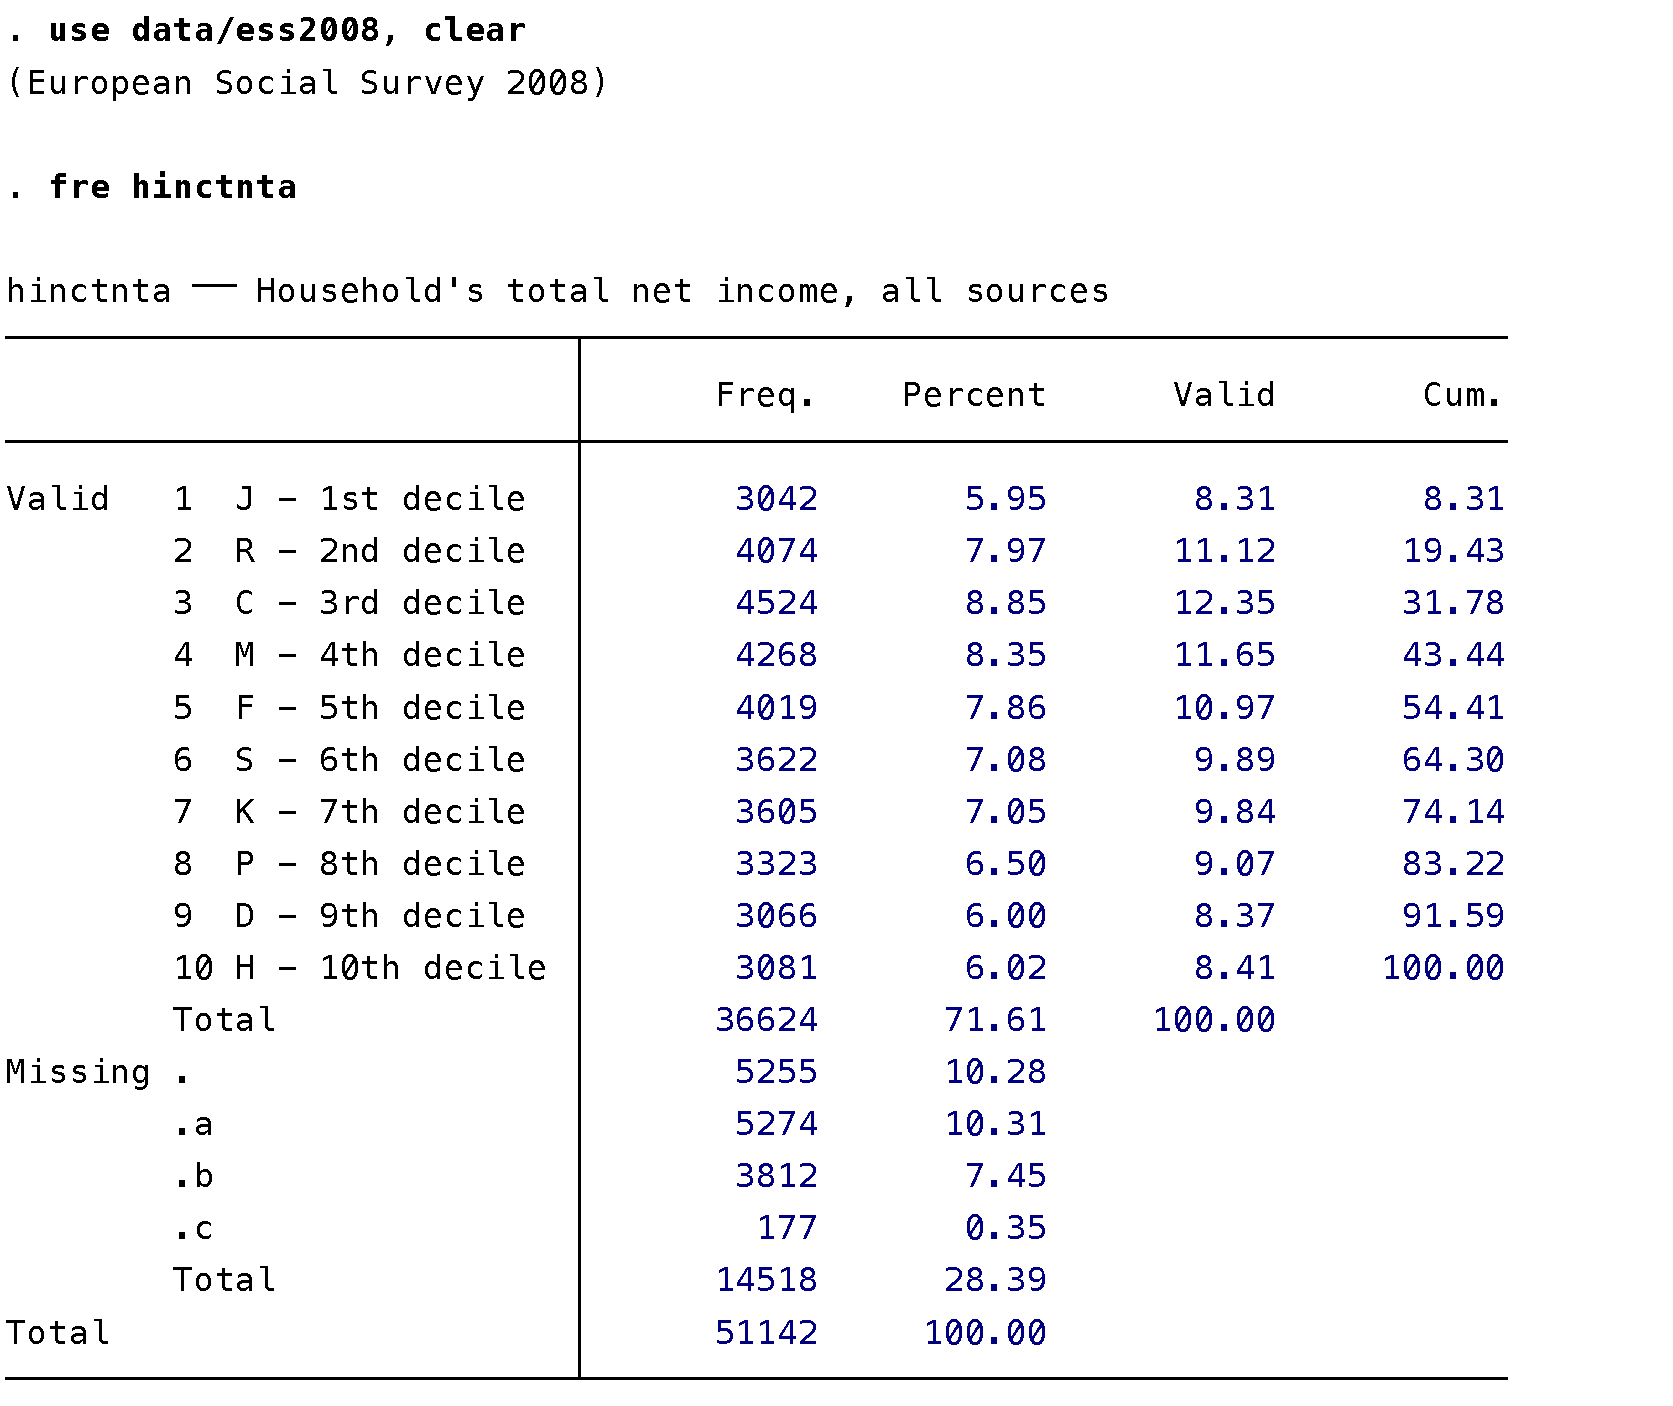
\includegraphics{ess-fre-hinctnta}\\[1em]
	
	Because the mean of a categorical variable does not reflect a true unit of measurement, it is not a useful descriptor: `the average age group is 4.5' is not a helpful statement. However, `the median age group' or `the modal age group' can be meaningful. This is because categorical variables can be described through \emph{relative frequencies}--generally \emph{percentages} (`40\% of political regimes are dictatorships') or \emph{fractions} (`half of the respondents are religious').

	In a categorical variable, the fraction of the sample taken by a category is its \emph{probability of occurrence}: if 45\% of the respondents are married, then the probability of being married among the respondents is $Pr(\mathrm{married}) = 0.45$. This is because categorical variables are best handled by thinking in terms of discrete probabilities: `percentages' are technically \emph{conditional probabilities}, and in a table, cell percentages are \emph{joint} probabilities and row or column percentages are \emph{marginal} probabilities.

	In the example below, \ess respondents were asked their feelings about their current household's income:\\[1em]
	
	\begin{docspec}
		use data/ess2008, clear\\
		fre hincfel
	\end{docspec}
	
	The largest group of respondents (the modal group), with 43\% of all responses, answered that they are `coping on present income'.\footnote{This group is also the group that contains the median respondent.} Since about 30\% of all respondents selected one of the last two response items, the probability for having difficulties living on current houseshold income is about $0.3$ among the (unweighted) sample of respondents:\\[1em]
	
	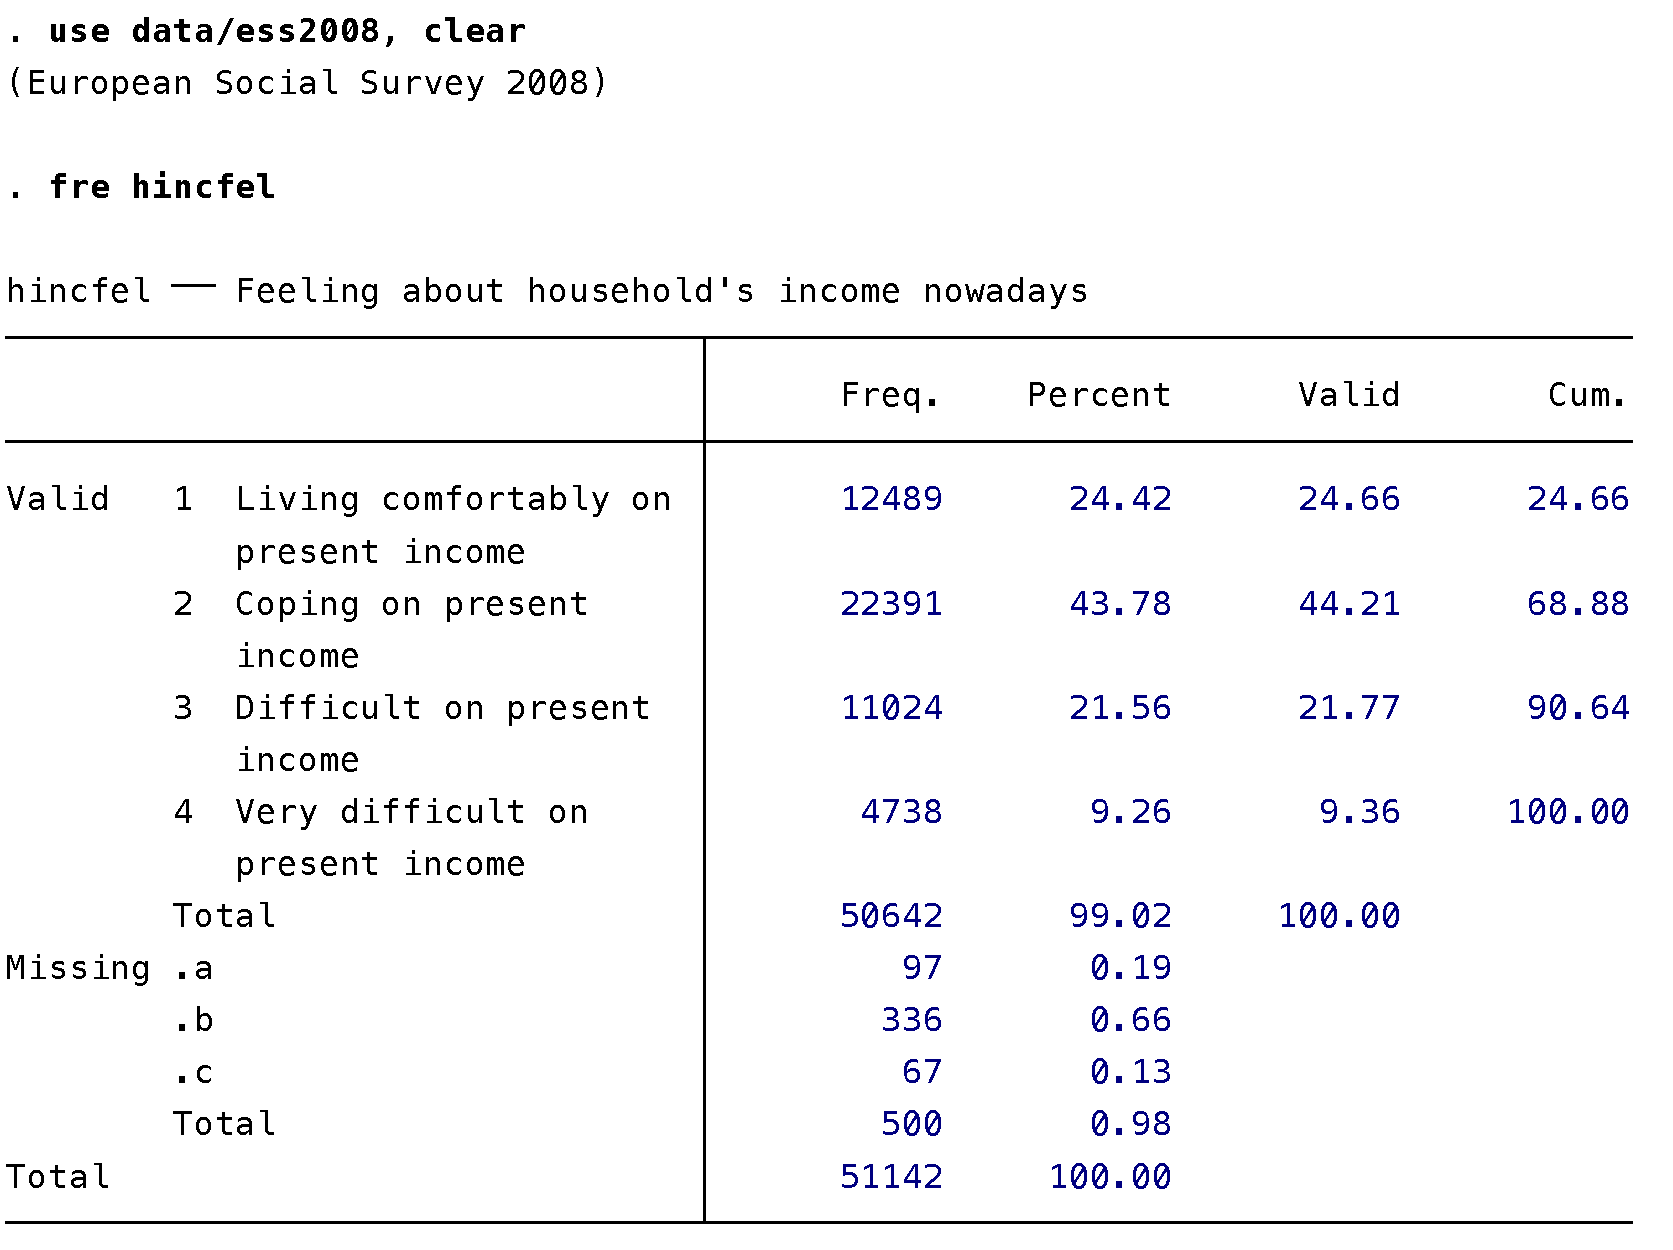
\includegraphics{ess-fre-hincfel}\\[1em]
		
	\index{Variables!Dummies (binary variables)}%
	\item[Dummies, or binary variables,] are categorical variables of the lowest possible dimensionality: they take only two values and therefore assert a logical statement: YES/NO, TRUE/FALSE, 0/1, male/female, married/single, democratic/dictatorial, etc. A convention is to name dummies after their true statement: a gender dummy called \texttt{female} codes 0 for `male' and 1 for `female'.
	
	The mean of a dummy is the fraction of the sample for which the logical statement is true. For example, if you code a dummy that holds 1 for `unemployed' and 0 for `employed' and the mean of that dummy, called \texttt{unemployed} so that its name denotes the true statement, is 0.18, then 18\% of the respondents have been reported or self-reported as unemployed (and the probability of being unemployed among the respondents is $Pr(\mathrm{unemployed}) = 0.18$. Dummies are particularly handy because of these `logical immediacy' characteristics.
	
	Here is an example of a \QOG dummy variable that codes for democratic status:\\[1em]
	
	\begin{docspec}
		use data/qog2011, clear\\
		fre chga\_demo
	\end{docspec}
	
	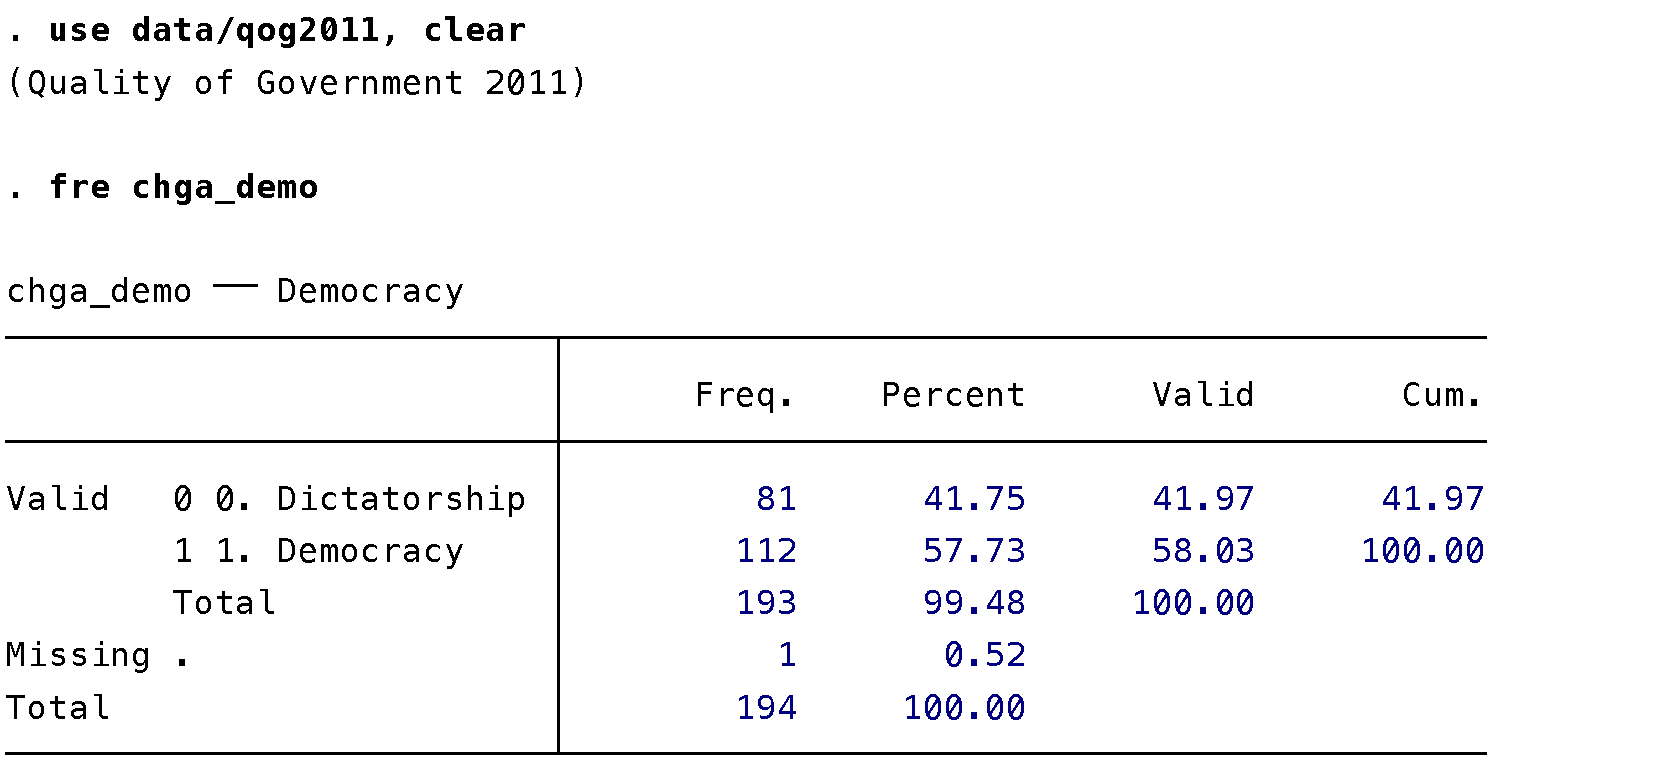
\includegraphics{qog-fre-chga_demo}\\[1em]
	
	In the example above, the variable could simply be renamed \texttt{democratic} and make immediate sense to the reader. It however often happens that dummies will be encoded as two `bland' items instead of having a logical sense, as in this \gss example:
	
	\begin{docspec}
		use data/gss2010, clear\\
		fre sex
	\end{docspec}
	
	It would be a good idea, in this case, to generate a meaningful dummy out of the existing one, using a logical statement to define the dummy, and excluding missing values from the process:%
		\label{female-dummy}
	
	\begin{docspec}
		* Create a female dummy.\\
		gen female:female = (sex == 2) if !mi(sex)\\[1em]
		
		* Label the values of the dummy.\\
		la def female 0 "Male" 1 "Female", replace\\[1em]
		
		* Check result.\\
		fre female
	\end{docspec}

	This example, which also appears in a Stata handbook by \cite{LongFreese:2001a}\footcite{FeinsteinThomas:2002d}, anticipates what we learn to do in the next sections with conditional statements, missing values and value labels. It takes the value 0 for males and 1 for females for nonmissing values of the \texttt{sex} variable, and then defines each value of the dummy through the \texttt{female} value label that has been assigned to the \texttt{female} dummy by the previous \cmd{gen}{generate} command:\\[1em]
	
	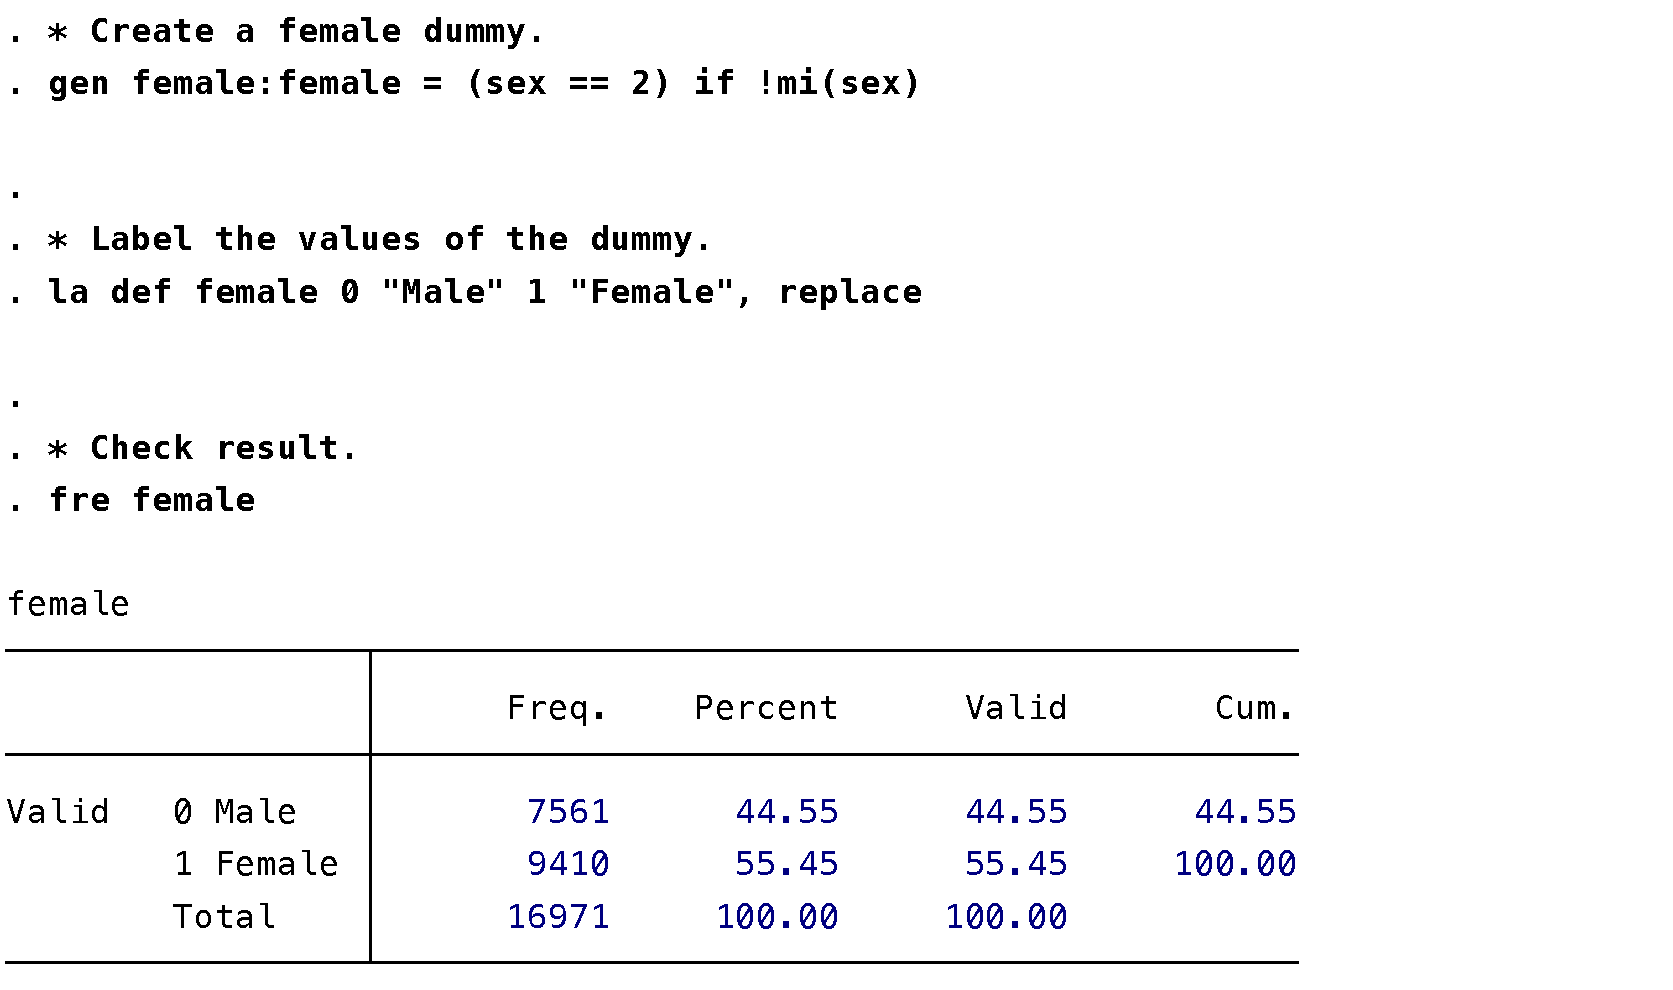
\includegraphics{gss-female-dummy}
	
	The percentages of a dummy are intuitively connected to its mean. If males are coded 0 and females 1, then the mean of the \texttt{female} variable is simply the ratio of females in the sample. The \cmd[su]{summarize} command provides the quickest way to compute this mean:
	
	\begin{docspec}
		* The mean of the dummy is the percentage of females.\\
		su female
	\end{docspec}

	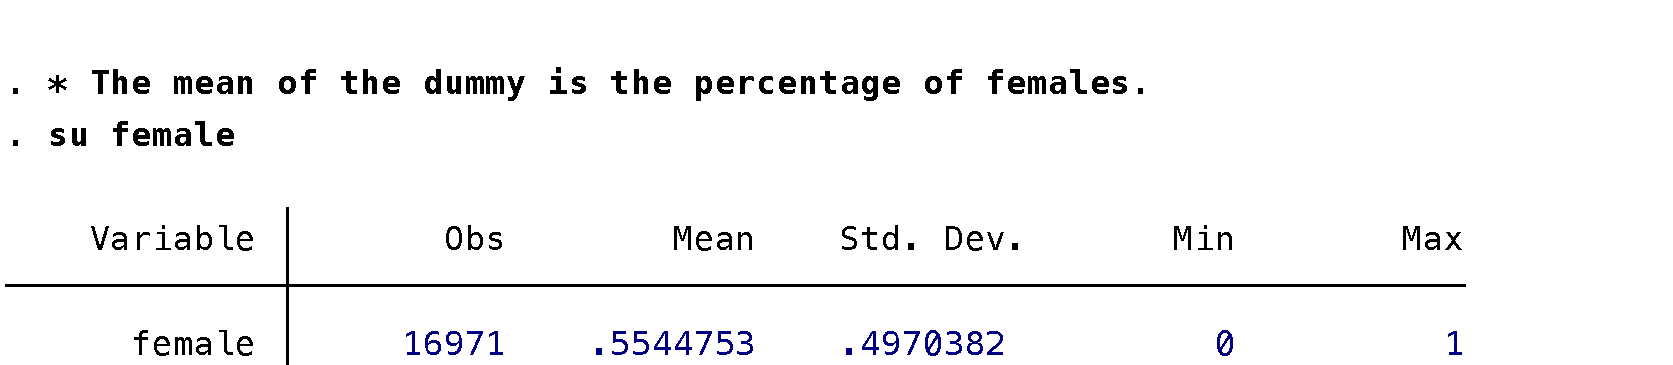
\includegraphics{gss-female-mean}
	
	The unweighted years of \GSS data used in the course have a slight excess representation of females, which is not unusual in survey data. This could be corrected, as most of our estimates could be, by using survey weights and a more complex survey design, set with the \cmd{svyset} command. The crude estimate, however, is generally enough for our purposes.\\[1em]

\end{description}

\newthought{Schematically}, continuous variables have mostly quantitative properties (meaningful units, infinite values, …), and categorical variables have mostly qualitative properties (their numbers code substantive groups or categories), whereas dummies have mostly logical properties.

You want to remember that terminology to understand what kind of distribution and summary statistics are appropriate to describe each type of variable, and then later how to plug each type of variable into a statistical test or model.

Accept some flexibility in classification: `continuous' and `categorical' denote abstract properties. Any physical variable is only imperfectly continuous from a mathematical perspective, and many ordinal variables with a large number of categories can be treated as continuous in practice.

Before you even start worrying about recoding continuous to categorical variables, let's cover missing values, as they work (almost) identically for all variables.

%
%
% 1.2 ==========================================================================
%
\subsection{Missing values}
\label{sec:missing-values}

\newthought{Missing values} are a consequence of survey nonresponse, coding errors and insufficient data. They might be coded with acronyms like `DK' (``don't know'') or `NA' (``no answer'' or ``not applicable''), or with numeric codes like -1 or 99. Observations that have missing values cannot be considered for the kind of analysis that we will later run, and we will eventually have to subset the data to exclude them from the sample.

\newthought{Stata requires missing values to be encoded} as dots ("\texttt{.}") that can be followed by a letter, as in "\texttt{.a}", "\texttt{.b}", ..., "\texttt{.z}". Any other value coding for missing values in the data has to be correctly recoded to `dot' encoding before the data is to be used in Stata, or summary statistics (among other things) will be wrongly reported. We show three different ways to recode missing values below.

\begin{description}
	\item[Selectively cloning a variable]%
	%
	A simple case of a missing value recode is when a variable needs to get trimmed from badly encoded missing values. Below is an example from the \NHIS dataset, where the last value for marital statuts is actually a missing value:

	\begin{docspec}
		use data/nhis9711, clear\\
		fre marstat
	\end{docspec}

	The issue is easy to diagnose with the \cmd{fre} command. It takes two built-in commands, \cmd[tab]{tabulate} and \cmd[la li]{label list}, to get the same output, so \cmd{fre} is always worth using to look at variable encoding:\\[1em]

	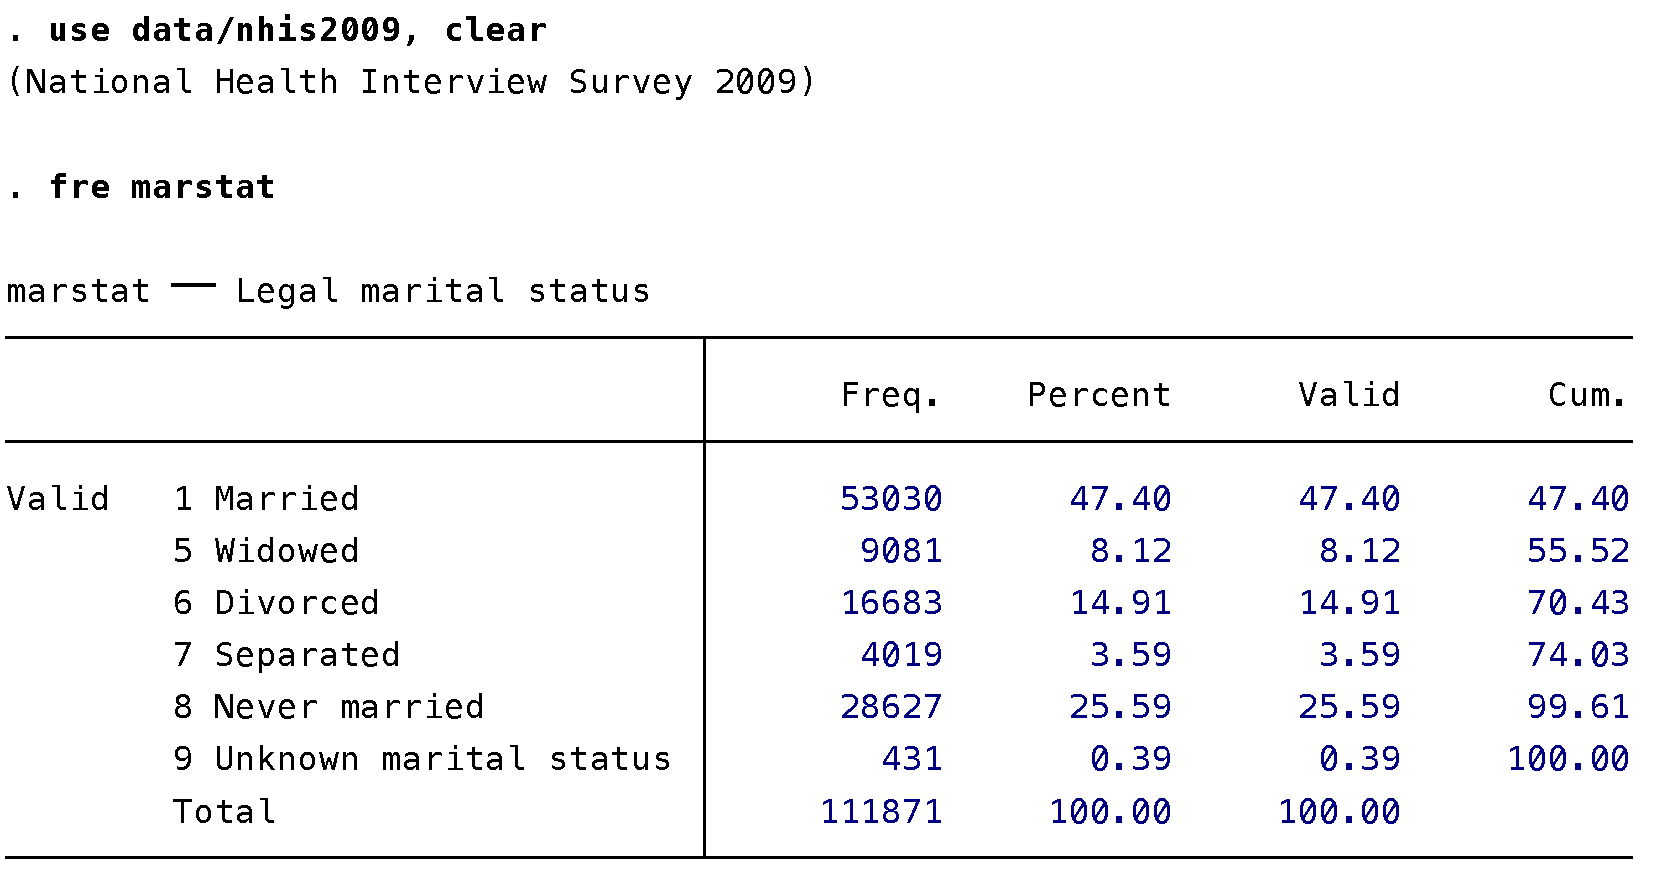
\includegraphics{nhis-fre-marstat}\\[1em]

	When the variable has labels that you want to preserve, the \cmd{clonevar} command lets you exclude the missing values and copy exactly everything else from the old variable to a new one, as shown below where we create the \texttt{marital} variable:

	\begin{docspec}
		clonevar marital = marstat if marstat < 9\\
		fre marital
	\end{docspec}

	All values and value labels (`Married', `Widowed', etc.) have been preserved in the new variable, at the exception of the 431 respondents of unknown marital status, who are now identified as missing by Stata:\\[1em]

	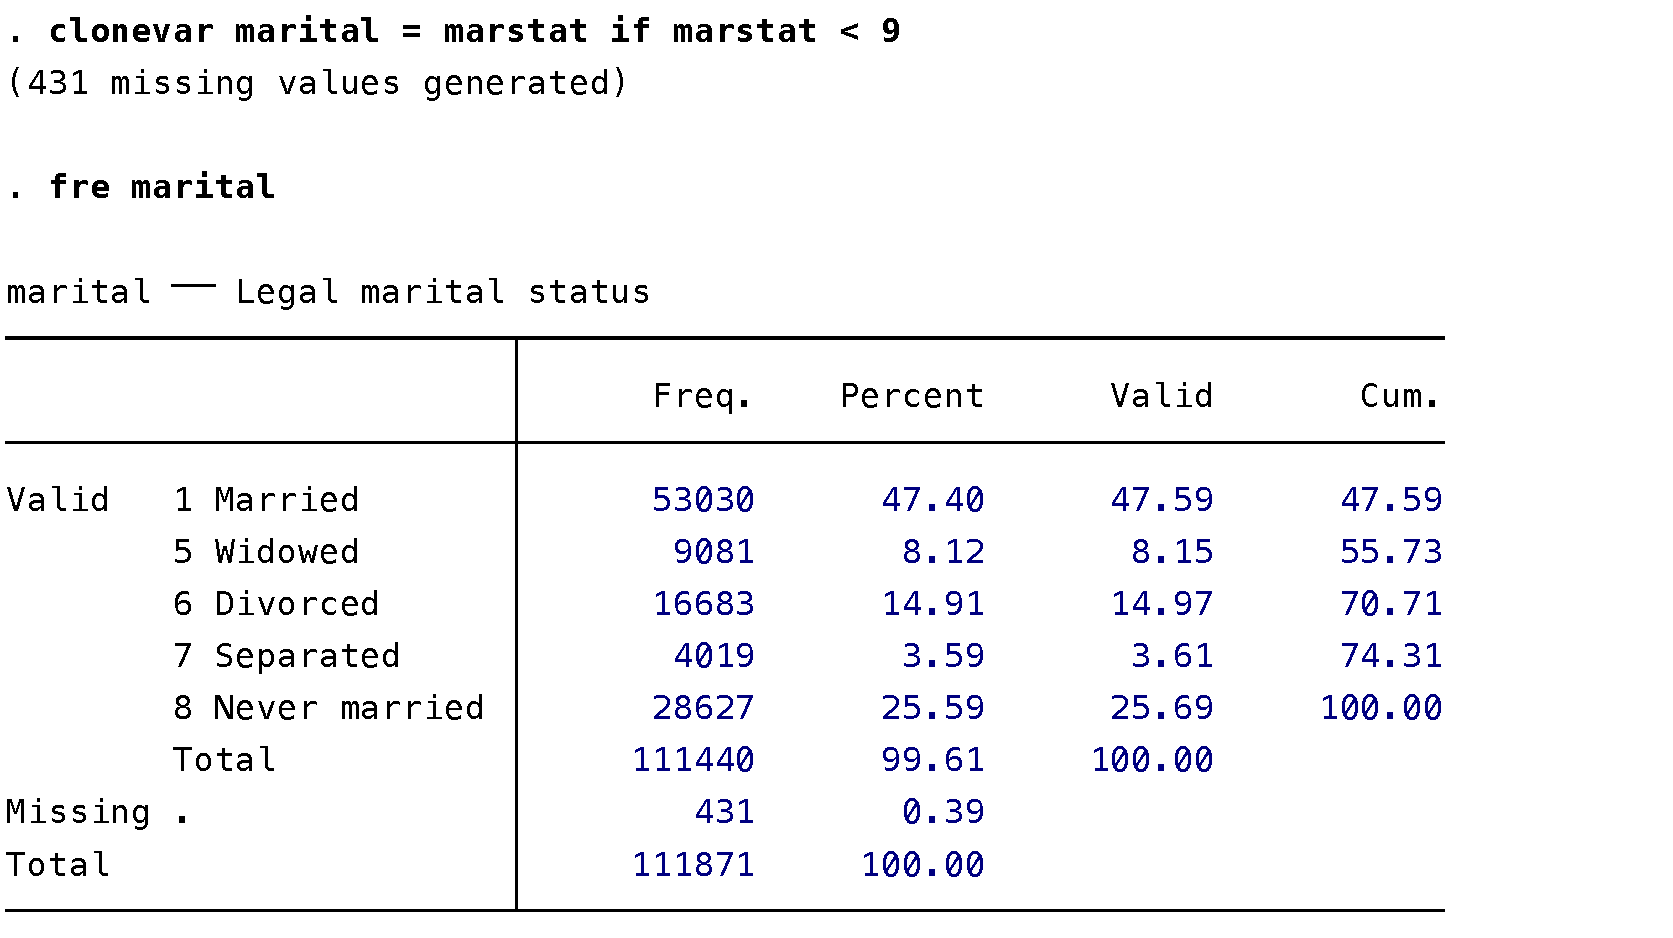
\includegraphics{nhis-clonevar-marital}\\[1em]

	\item[Selectively duplicating values]%
	%
	When the variable does not have labels, you can be most straightforward and use the \cmd[gen]{generate} command to recode specific values to missing. Our example for such an operation shows the coding of the age variable in the \wvs:

	\begin{docspec}
		use data/ess0810, clear\\
		fre edulvla, nomissing nowrap
	\end{docspec}
	
	We use the \cmd{fre} command to diagnose the issue, passing the \coab{r}{rows}{fre} option in order to show only a few values instead of the full range from 15 to 99. Strangely enough, values 98 and 99 indicate missing data here:\\[1em]

		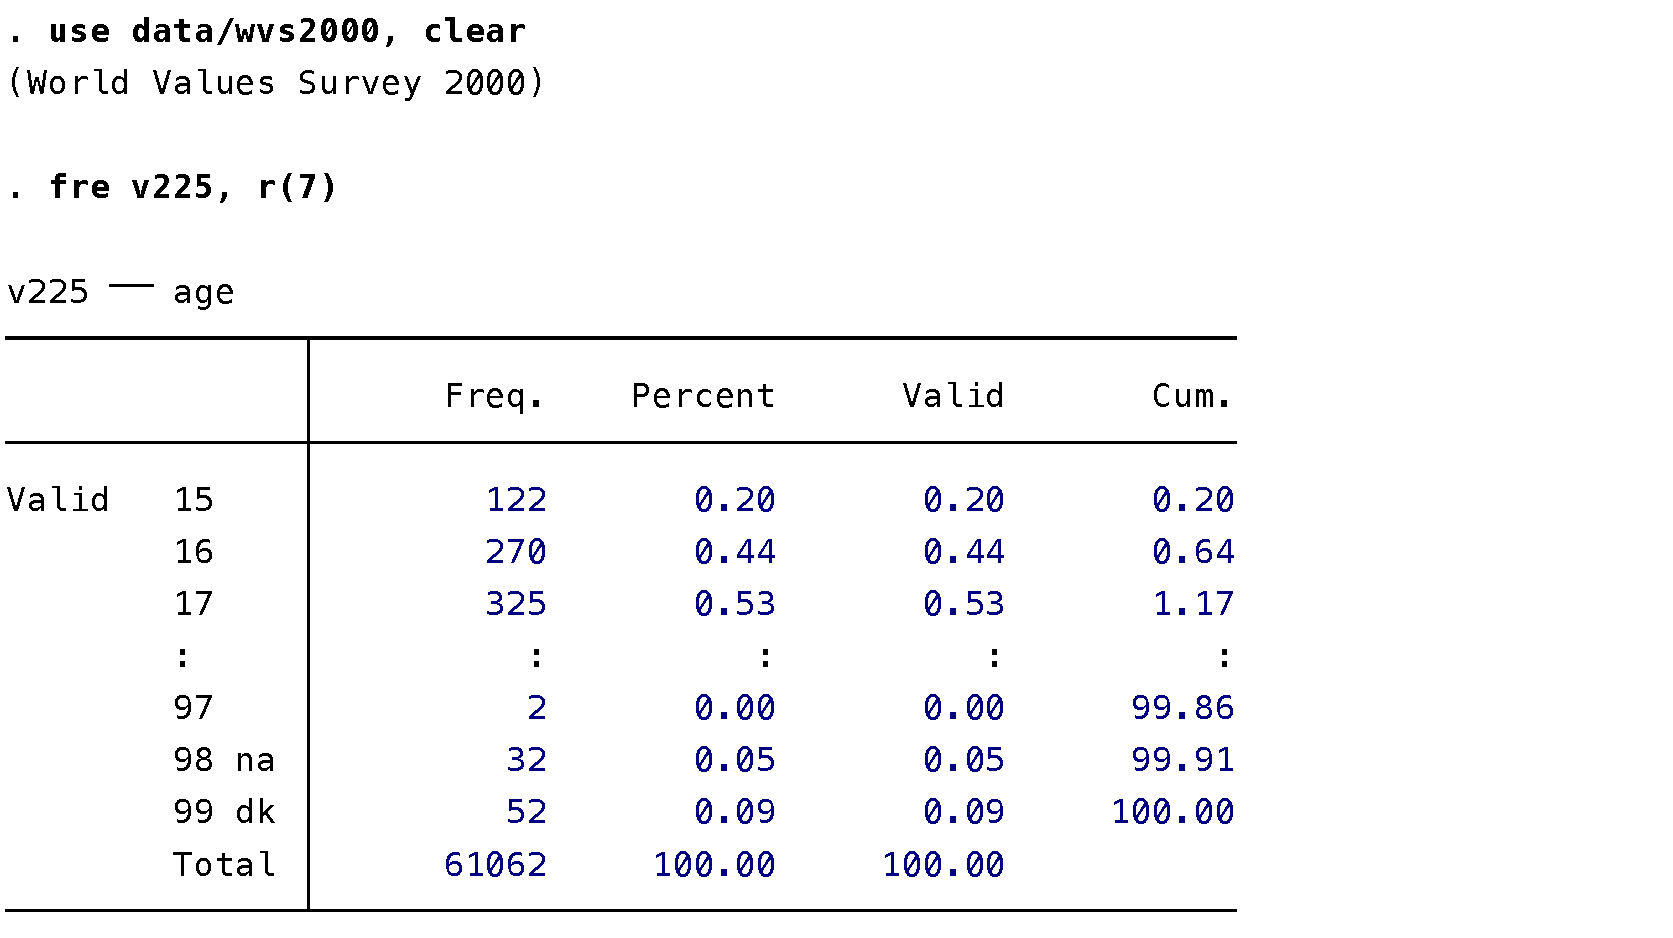
\includegraphics{wvs-fre-age}\\[1em]
	
	This error can be fixed simply by recomputing an age variable that excludes the upper categories with the \cmd[gen]{generate} command, which duplicates the nonmissing values and allows to pick up a better name for the variable all at once:

	\begin{docspec}
		gen edu = edulvla if edulvla < 55\\
		fre edu, nomissing nowrap
	\end{docspec}

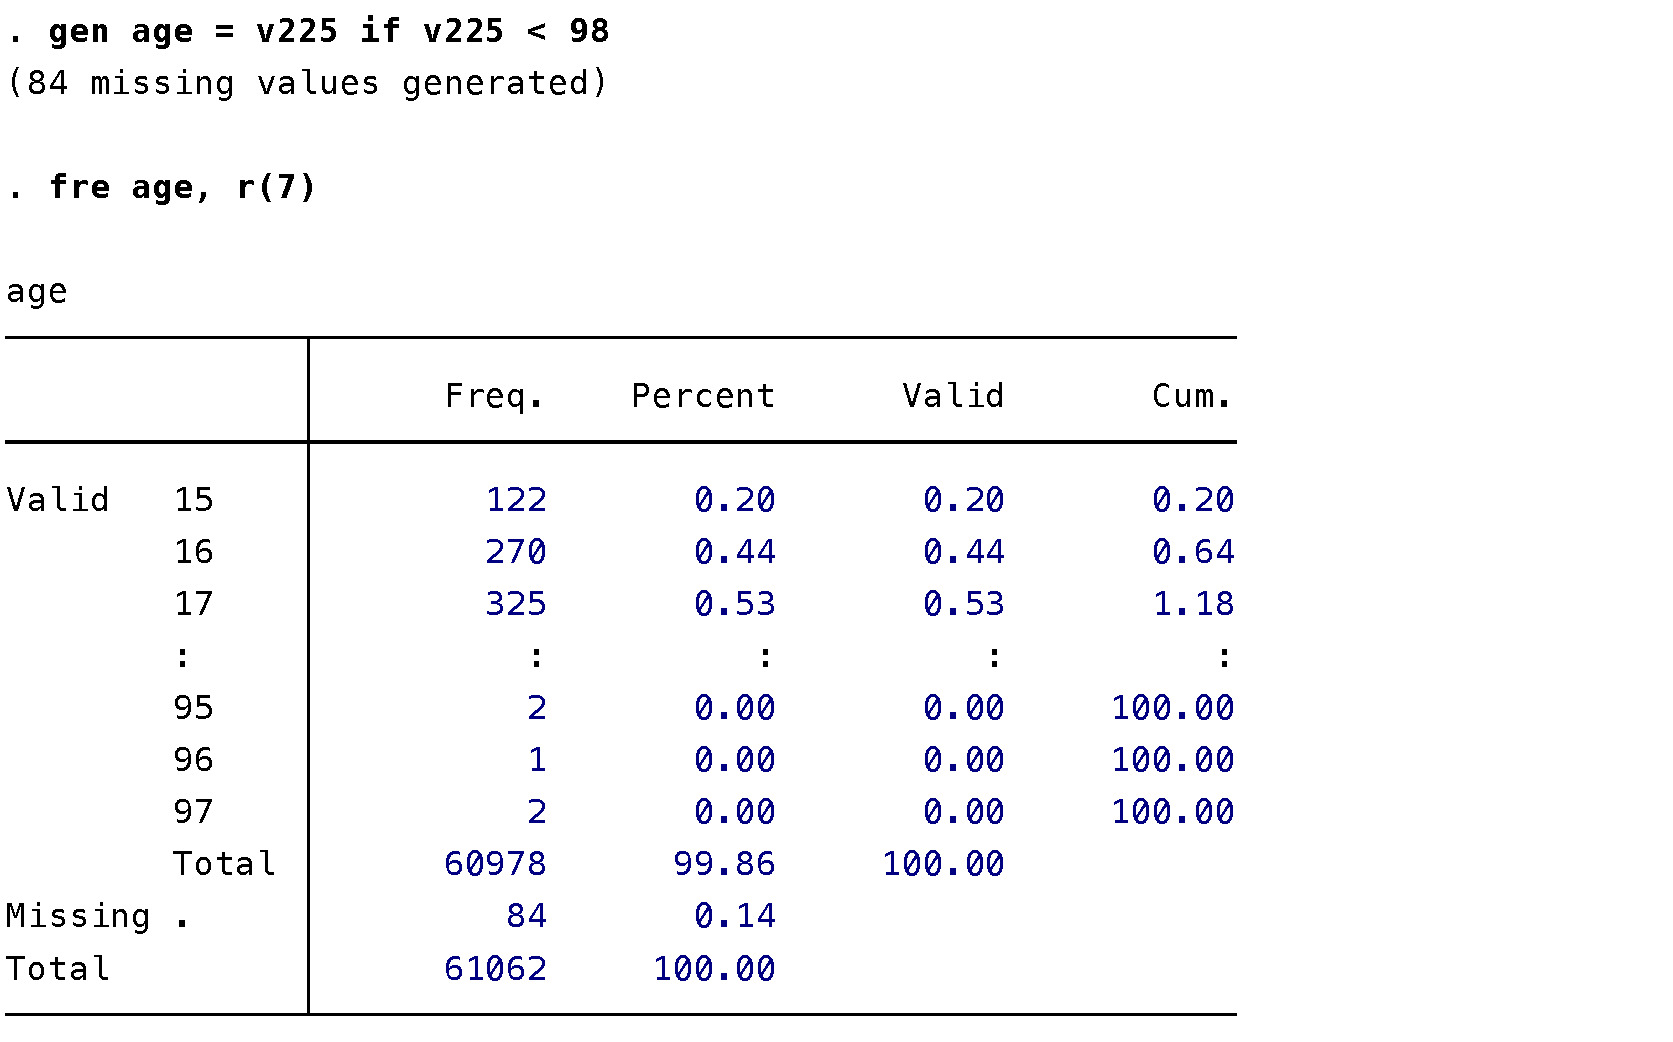
\includegraphics{wvs-gen-age}\\[1em]

	\item[Batch encoding of missing values]%
	%
	The \cmd{clonevar} and \cmd[gen]{generate} methods lose in efficiency if you are recoding missing values that follow the same coding scheme from one variable to another. The example below illustrates that situation with two \NHIS variables:\\[1em]

	\begin{docspec}
		use data/ess0810, clear\\
		fre edulvla eisced, nomissing nowrap
	\end{docspec}
	
	The \texttt{pooryn} and \texttt{uninsured} are both using \texttt{9} as a missing value.
	
	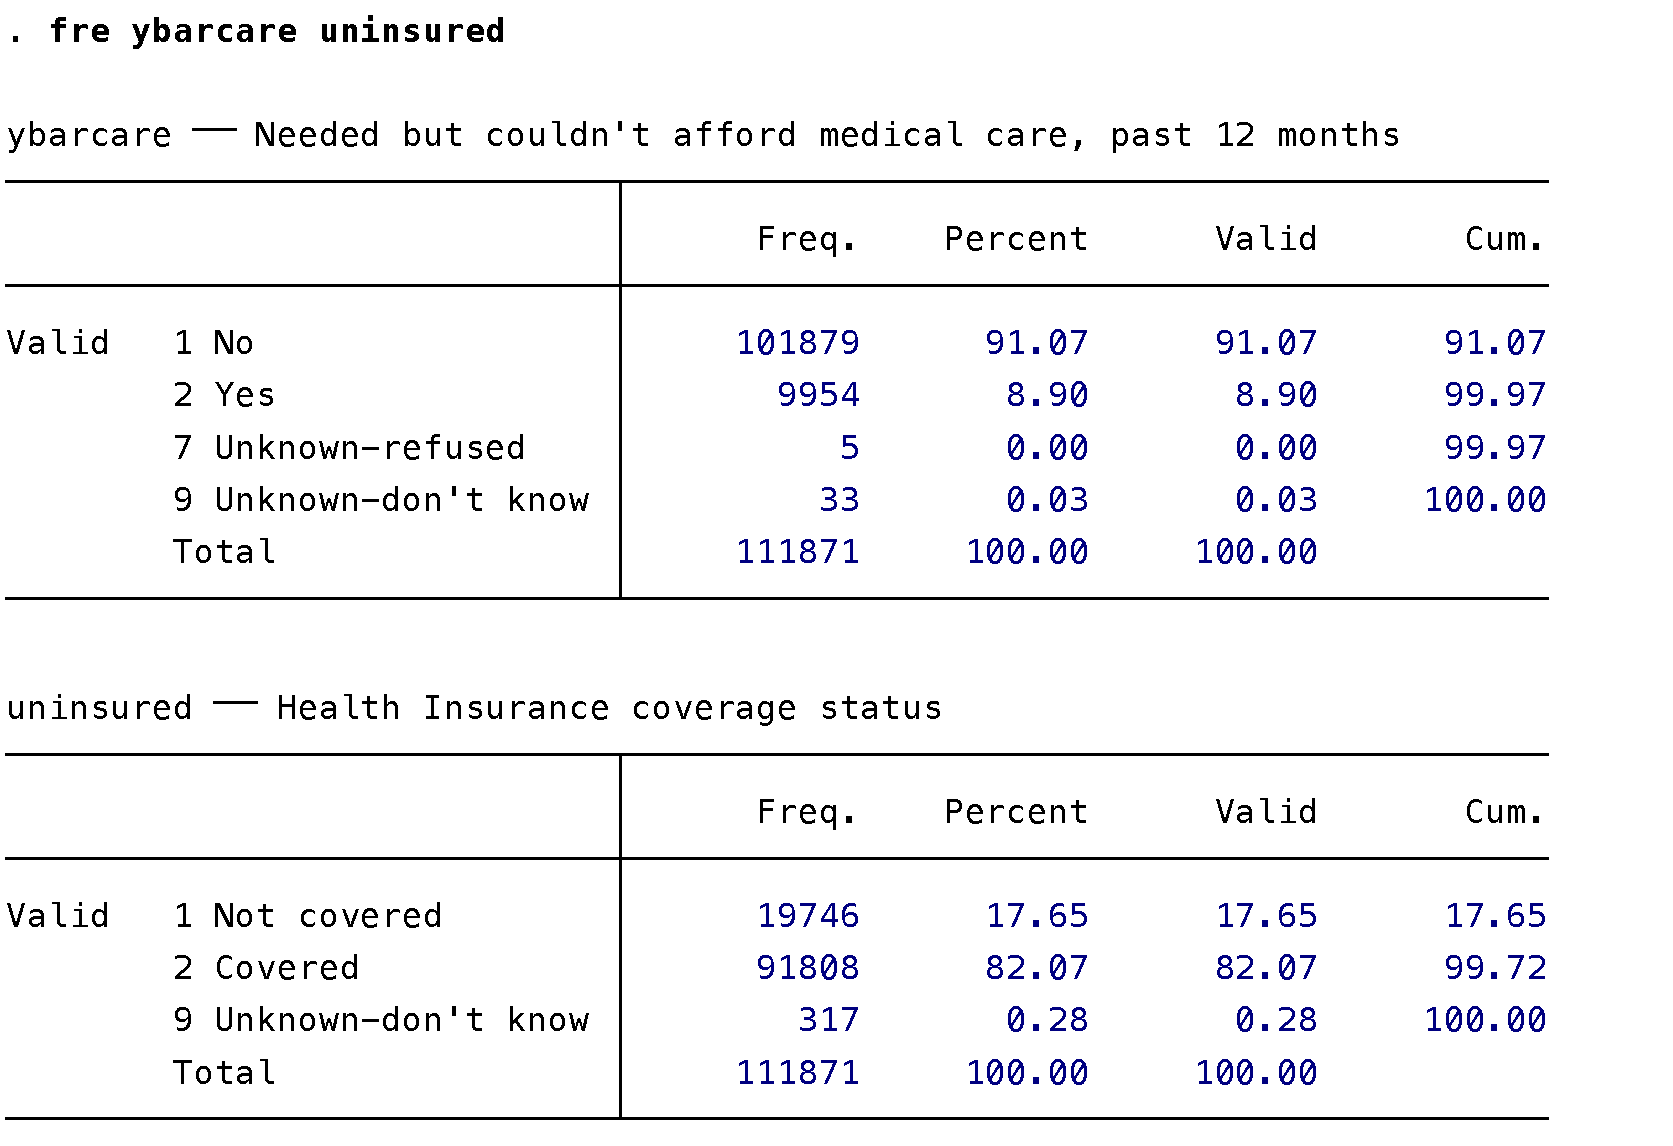
\includegraphics{nhis-fre-ybarcare-uninsured}\\[1em]

	In that case, the \cmd{mvdecode} command is quicker at coding these values to missing directly within the variables. The command works by specifying which variables are concerned, and what values should be recoded to missing:

	\begin{docspec}
		* Recode missing values of insurance and medical care.\\%
		mvdecode edulvla eisced, mv(55)\\[1em]%
		%
		* Check results.\\%
		fre edulvla eisced, nomissing nowrap\\%
	\end{docspec}
	
	Use this command with caution, as it makes it easy to recode erroneously, and systematically check your batch recodes:\\[1em]%

	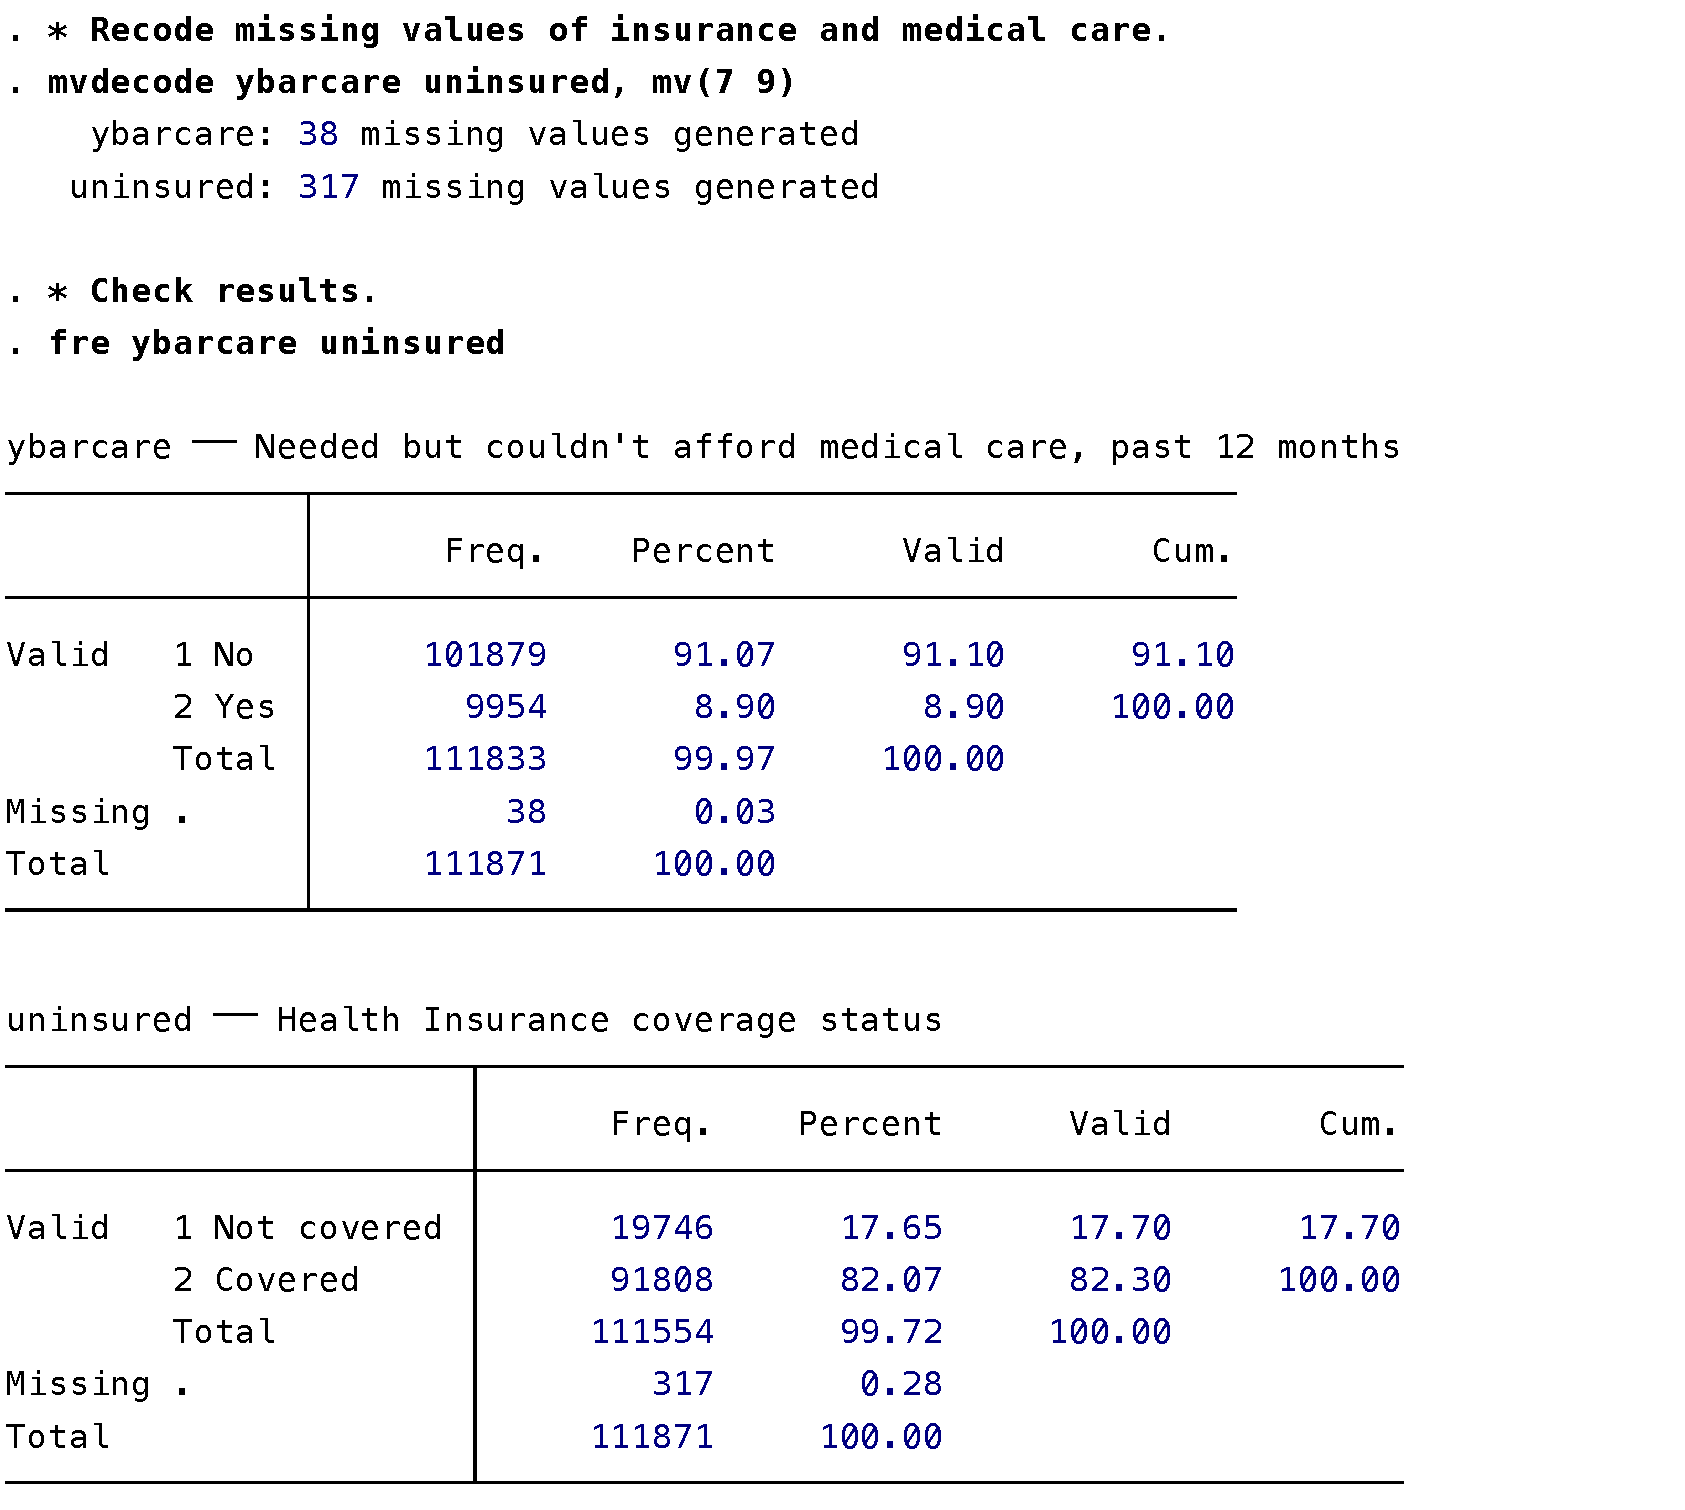
\includegraphics{nhis-recoded-ybarcare-uninsured}
\end{description}

\paragraph{Using logical operators} %
As previously with the female dummy recode from p.~\pageref{female-dummy} we have used a logical statement with the \cmd{if} command, to operate a command only for a selection of observations. The one above says: ``apply (the \texttt{clonevar} command) only to observations for which (marital status) is strictly inferior to 9''. A list of Stata logical statements is shown below:

\begin{table}
	\begin{center}
  	\footnotesize
  	\begin{tabular}{ll}
    	\toprule
    	Symbol & Meaning \\
    	\midrule
    	\quad \texttt{>} and\texttt{>=} & strictly superior / or equal to \\
    	\quad \texttt{<} and\texttt{<=} & strictly inferior / or equal to  \\
    	\quad \texttt{==} & equal to \\
    	\quad \texttt{!=} & \emph{not} equal to \\
    	\quad \texttt{mi(x, y, z)} & missing any of the variables\texttt{x, y, z}\\
    	\quad \texttt{!mi(x, y, z)} & \emph{not} missing any of the variables\texttt{x, y, z}\\
    	\quad \texttt{inlist(x, ...)} & values of variable \texttt{x} in the list \texttt{...}\\
    	\quad \texttt{if (...) \& (...)} & if (...) \emph{and} (...)\\
    	% \quad \texttt{if (...) | (...)}  & if (...) \emph{or} (...)
    	\bottomrule
  	\end{tabular}
	\end{center}
	\label{tbl:logical-symbols}%
		\index{Logical statements}\index{Selectors!Logical conditions: \cmd{if}}
\end{table}
	
\newthought{Once missing values are encoded}, you will have to subset your data, that is, to extract the set of observations for which no values are missing in the data. The \cmd{misstable pat} command provides a handy way to establish, as in the \ESS example below, the percentage of fuly measured observations:

	\begin{docspec}
		use data/ess0810, clear\\
		misstable pat agea gndr edulvla hinctnta
	\end{docspec}
	
	For the purpose of this example, the \cmd{misstable pat} command is shown immediately after data loading, but you should run it after recoding missing values to make sure that the subset works properly. The result is a table that provides the percentage of `full data' and indicates which variables have missing values:\\[1em]
	
	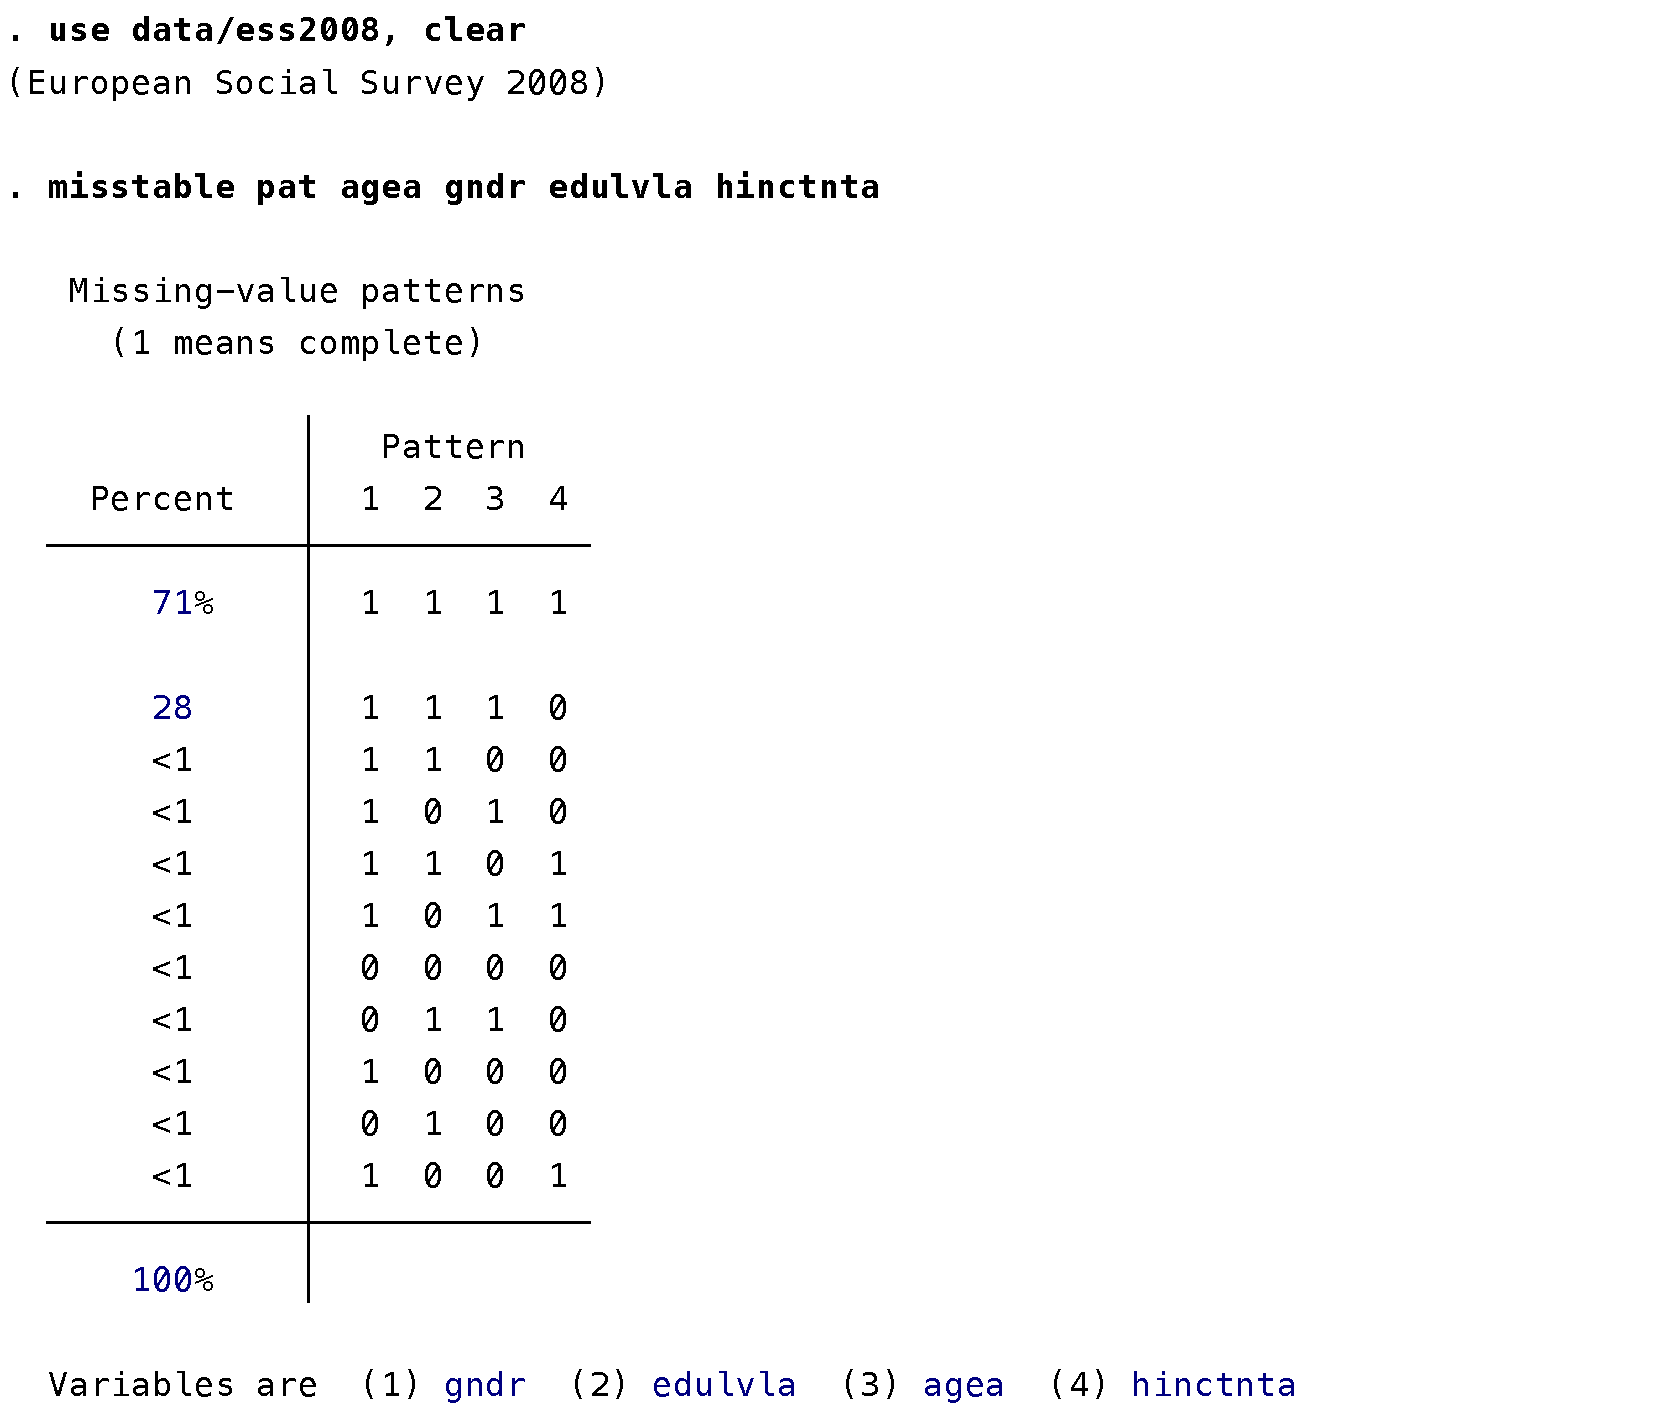
\includegraphics{ess-misstable-pat}\\[1em]

	The \cmd{misstable pat} command should be used at the right level of precision. For example, when working on comparative country case studies, you should specify each country separately to spot variations in missing values among the case studies:\\[1em]
	
	\begin{docspec}
		use data/ess0810, clear\\[1em]%
		%
		* Missing values for Germany.\\%
		misstable pat agea gndr edulvla hinctnta if cntry == "DE"\\[1em]%
		%
		* Missing values for Turkey.\\%
		misstable pat agea gndr edulvla hinctnta if cntry == "TR"
	\end{docspec}

	In this example, the country variable is not encoded but provided as text (string data) instead, which is why we can designate the countries directly by their acronyms between quotes:

	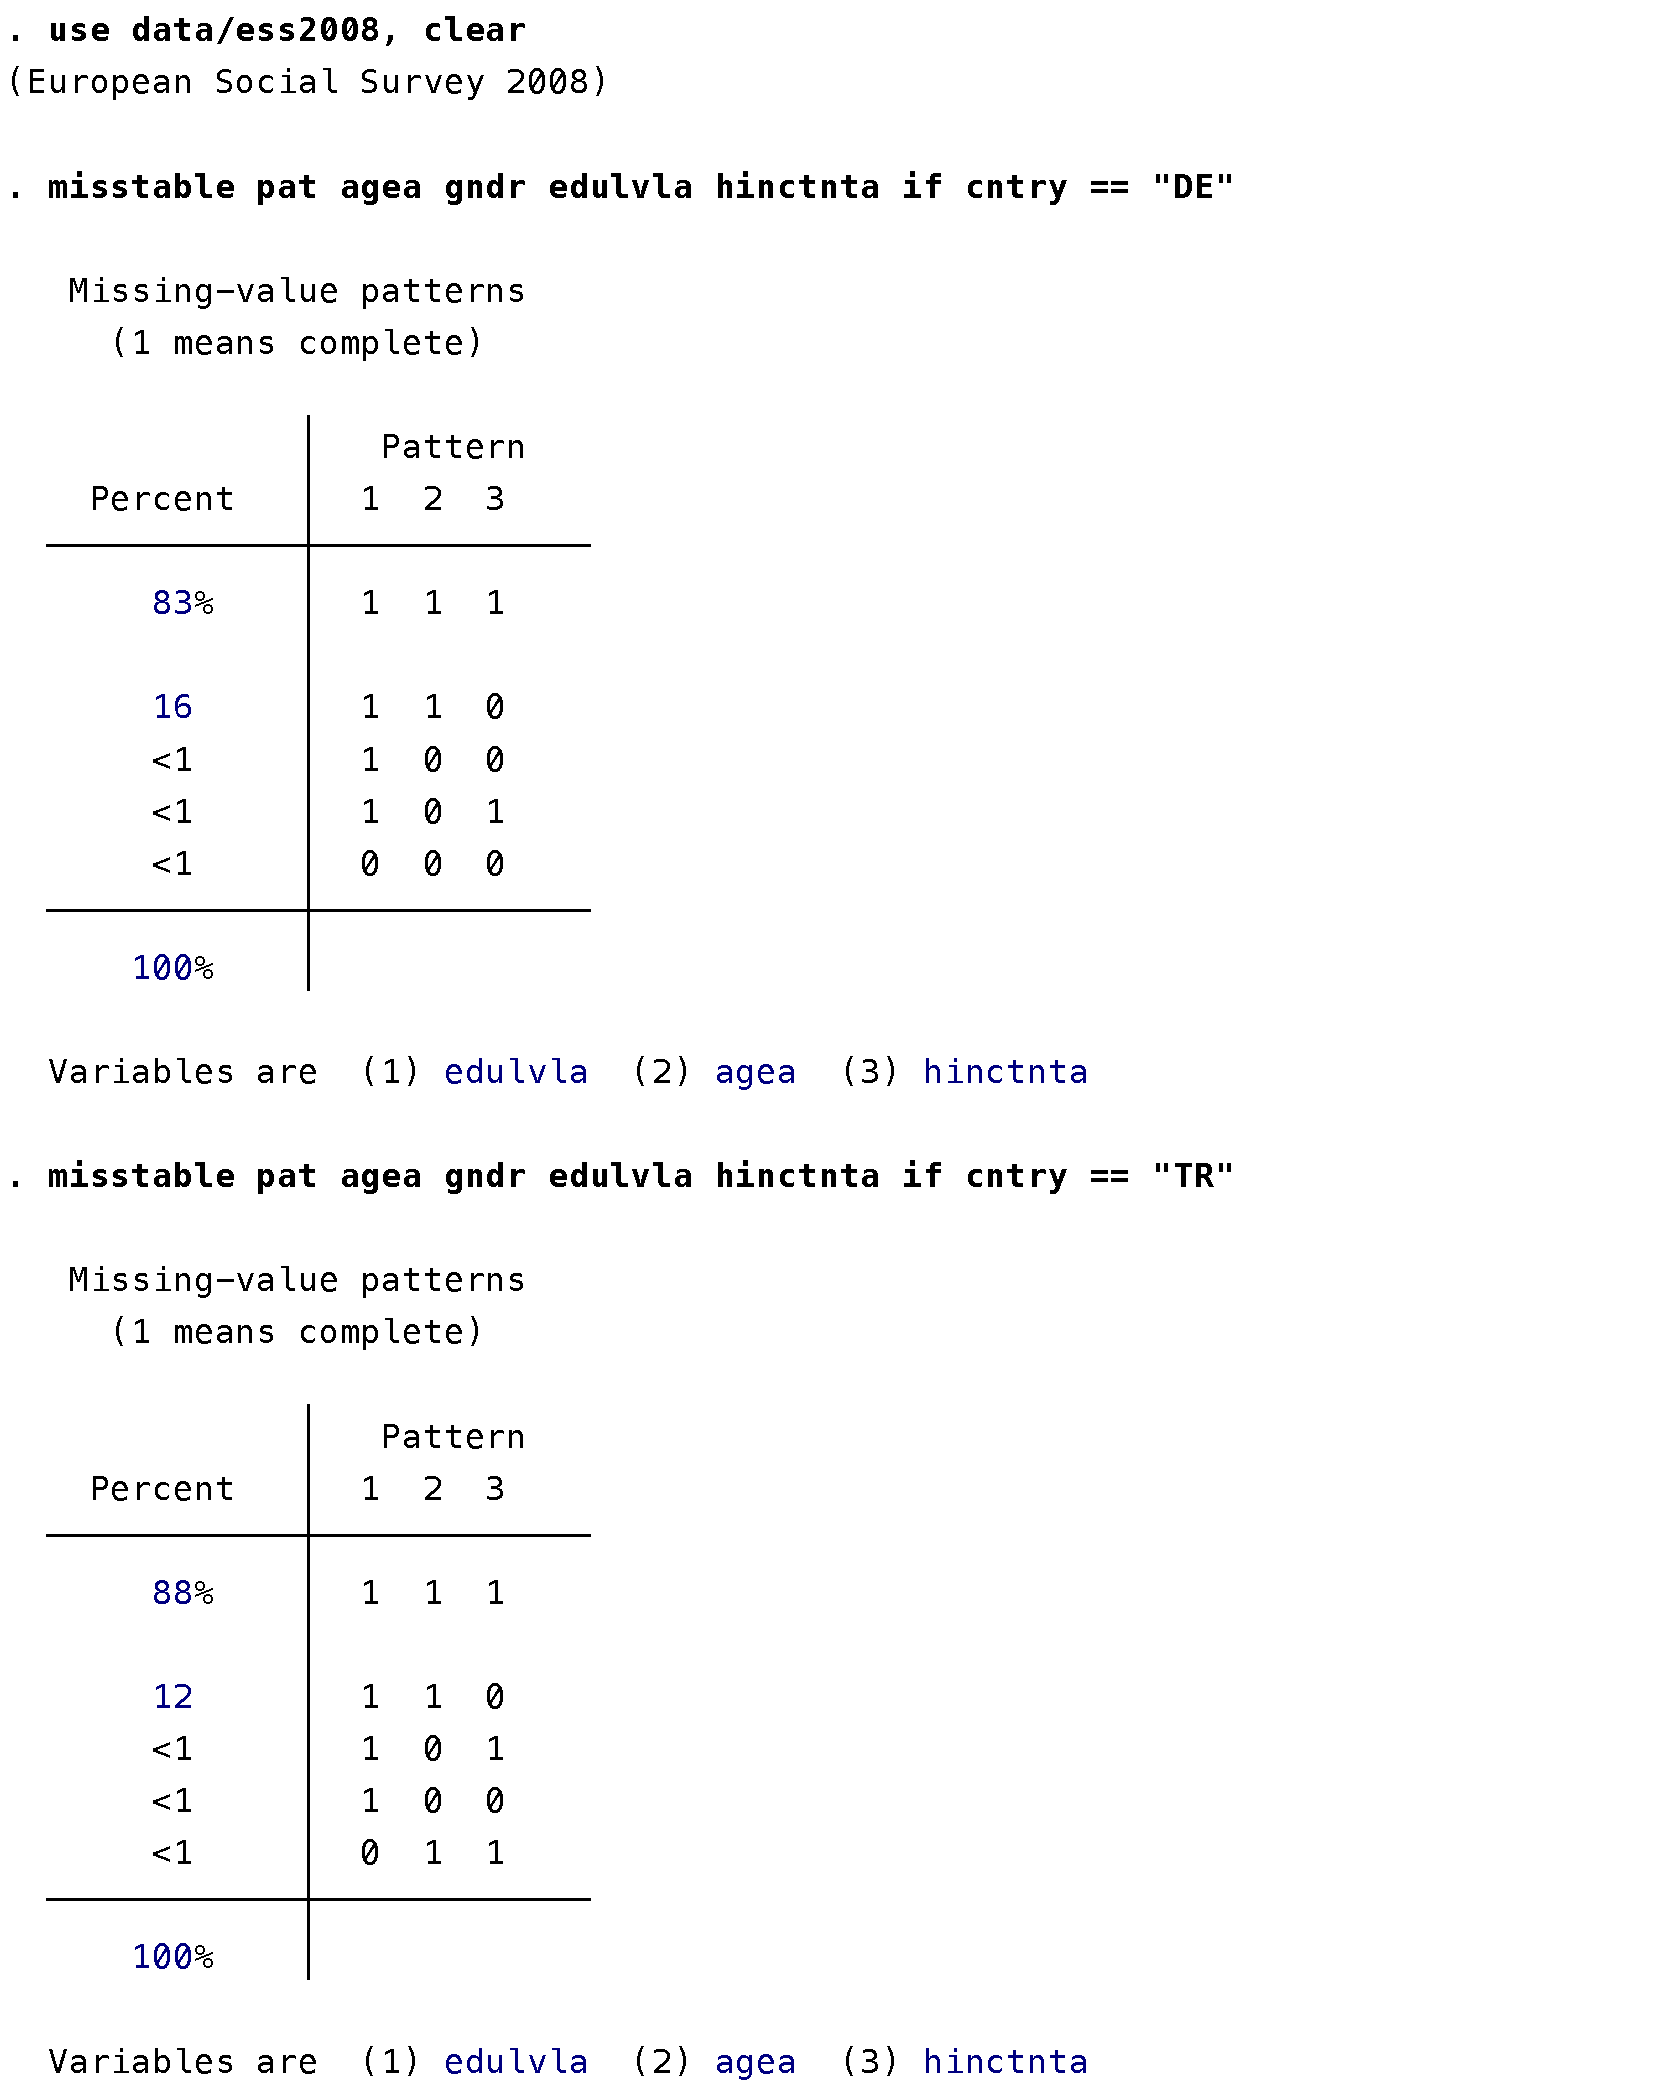
\includegraphics{ess-misstable-pat-cntry}\\[1em]
	
	Identically, on country-level data, you will also want to go a step further by inspecting the missing values more in depth. In this example, the \coab{freq}{frequency}{misstable} option shows the precise number of countries that would be left in the data with the following selection of variables:\\[1em]
	
	\begin{docspec}
		use data/qog2011, clear\\%
		* Missing values.\\%
		misstable pat wdi\_fr wdi\_gdpc bl\_asyt25 chga\_hinst\\[1em]%
		%
		* Missing values dummy.\\%
		gen missing = mi(wdi\_fr, wdi\_gdpc, bl\_asyt25, chga\_hinst)\\%
		* Geographic comparison.\\%
		table ht\_region, c(n missing mean missing)
	\end{docspec}
	
	The last lines of the code create the \texttt{missing} dummy equal, for each observation, to 1 if there is any missing data in the selected variables, and 0 otherwise. The mean of the dummy is then shown by geographical region, showing for instance that 93\% of the 29 East European and post-Soviet Union countries have missing data in the selected variables:\\[1em]
	
	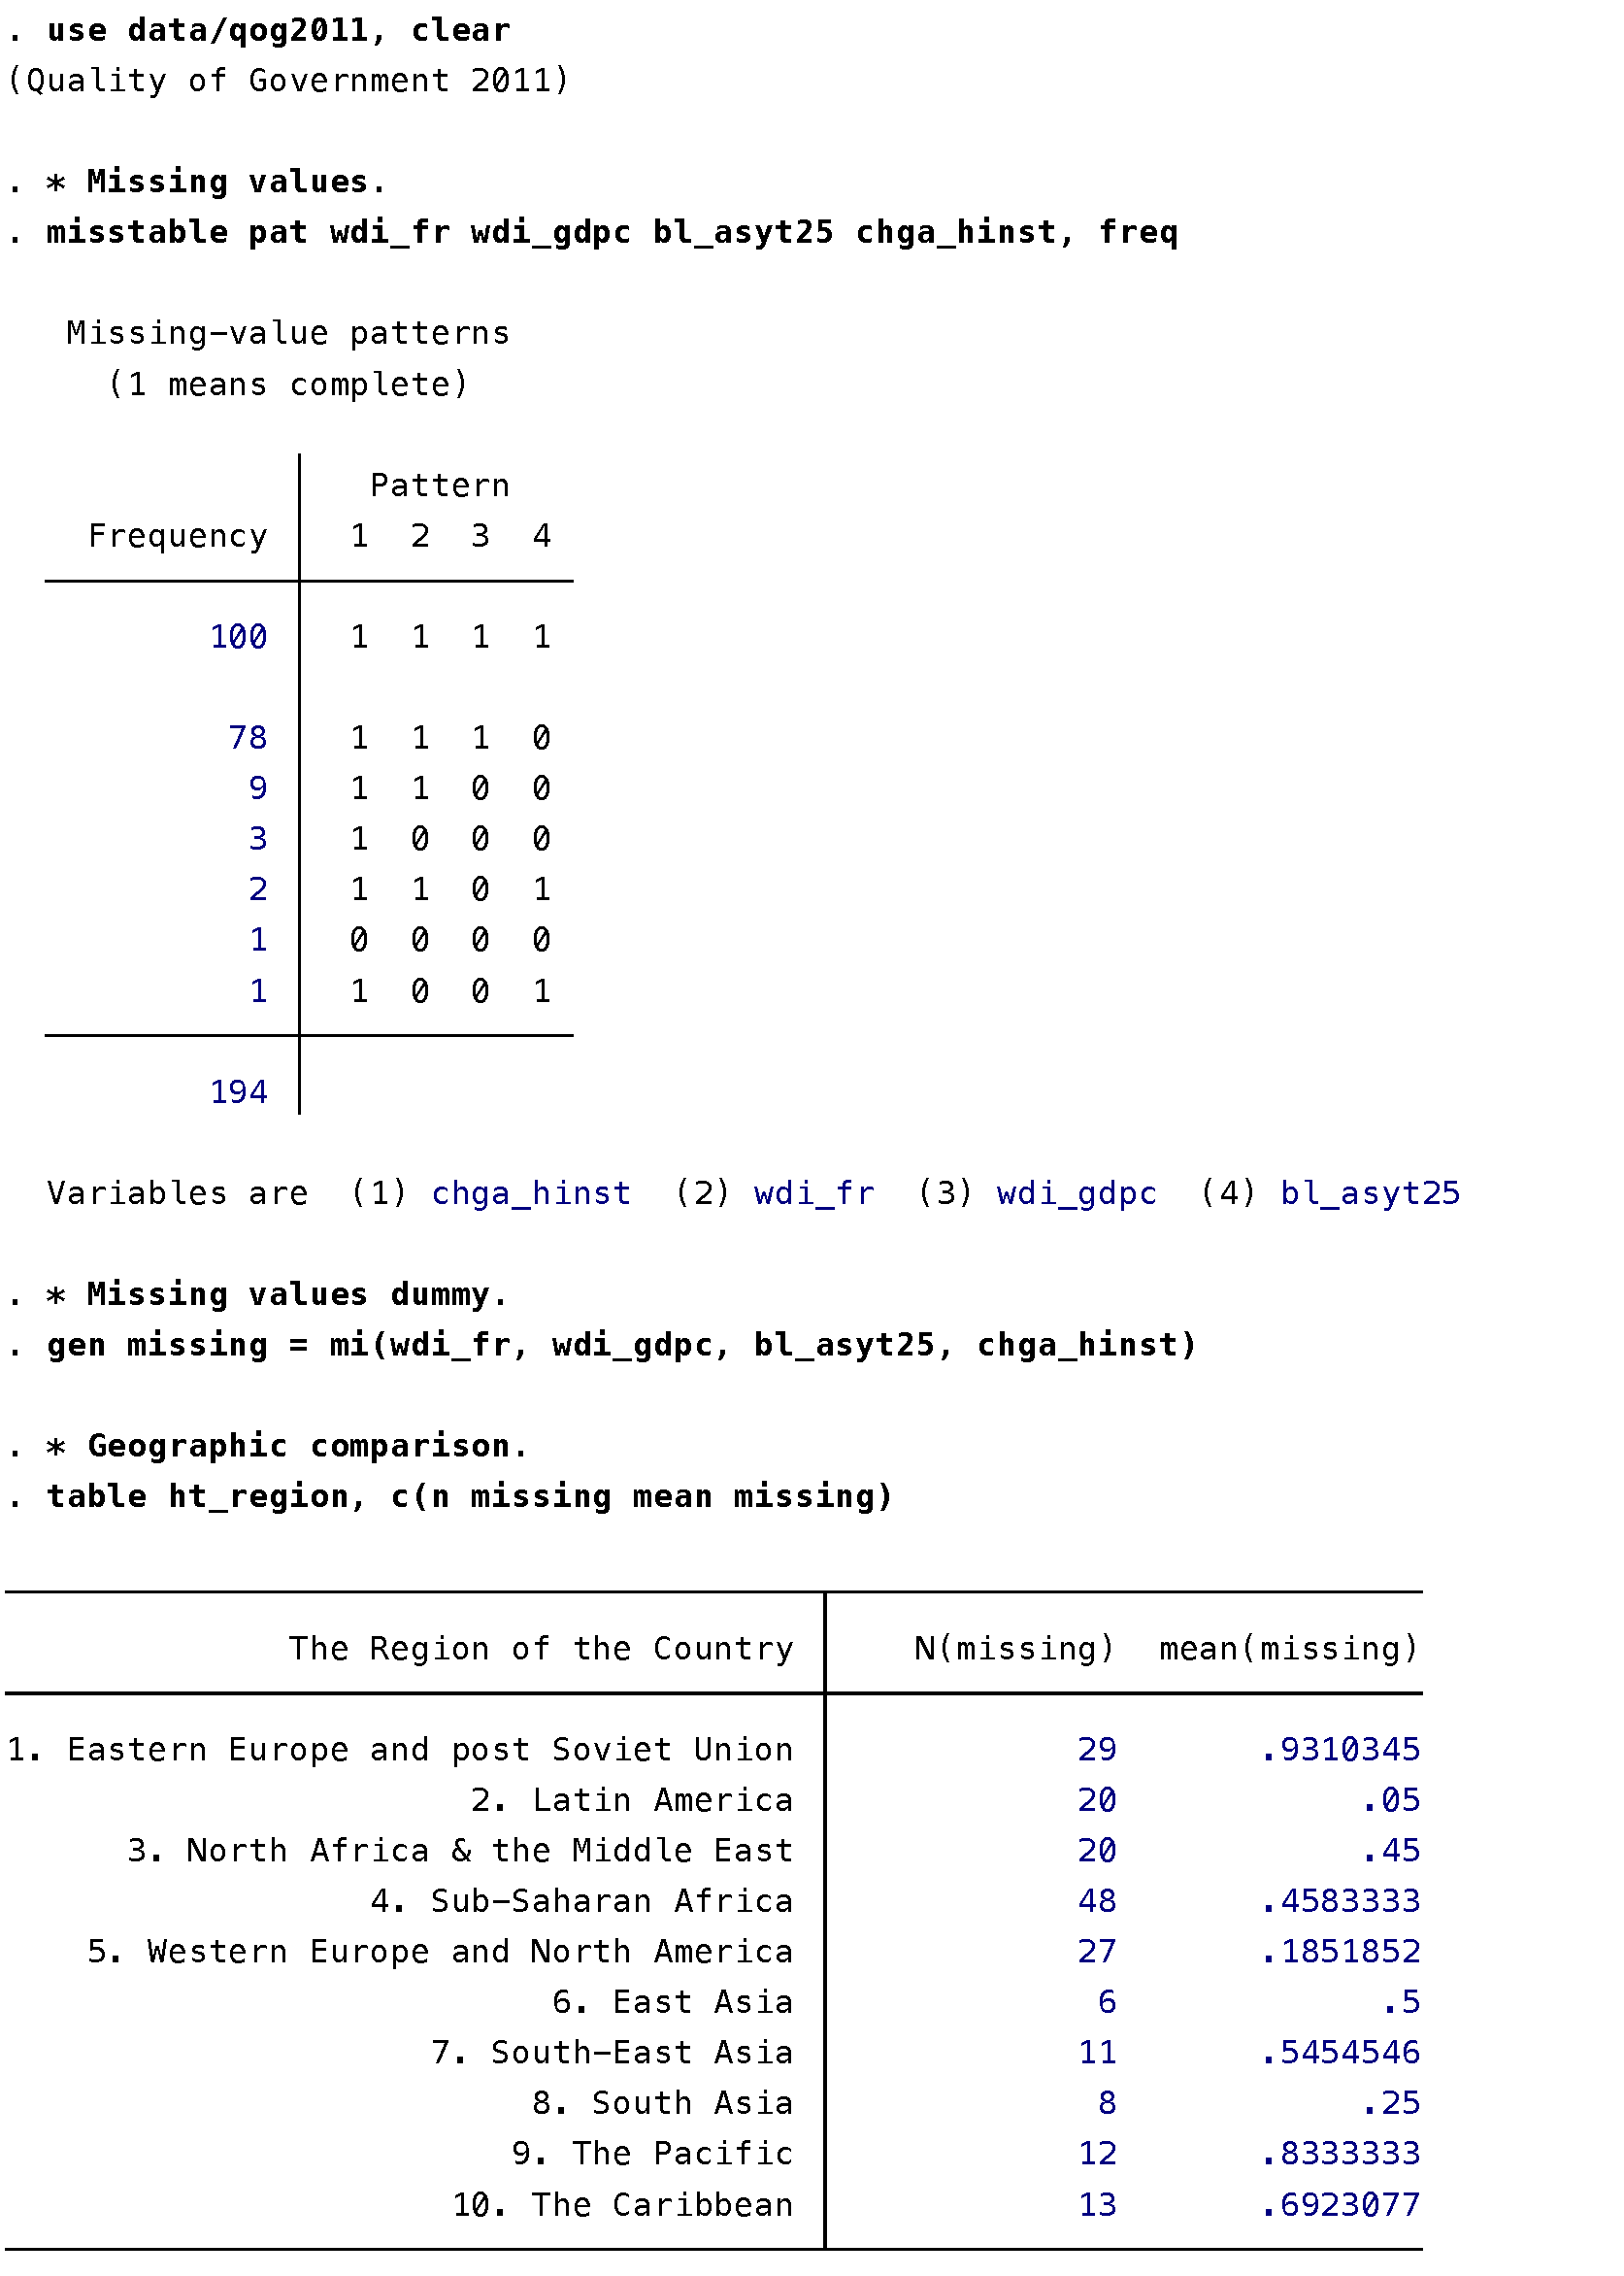
\includegraphics{qog-misstable-freq}\\[1em]
	
	\newthought{The amount of missing values in the data} becomes an issue when it starts affecting the representativeness of your sample, or when it simply falls too low for statistical tests to operate properly; the oft-cited threshold is around $N = 30$, but anything low is both a threat to external validity and a handicap for the subsequent analysis. 
	
	Your finalized sample is the sample left after subsetting to full data with the \cmd{drop} and \cmd{keep} commands. The example below subsets the \ESS data twice, first to keep only observations from two country case studies, then to delete observations with missing data:
	
	\begin{docspec}
		use data/ess2008, clear\\
		* Keep only Germany and Turkey.\\
		keep if inlist(cntry, "DE", "TR")\\
		* Remove missing data.\\
		drop if mi(agea, gndr, edulvla, hinctnta)
	\end{docspec}
	
	\newthought{What can be done about missing data} is a topic that goes beyond the scope of this class, into interpolating and, by extension, simulation. The conservative view that we adopt here for simplicity consists in recommending that the only cure for data is more data.

%% - missing values
%% misstable, drop, keep, count

%
%
% 1.3 ==========================================================================
%
\subsection{Categorical recodes}
\label{sec:categorical-recodes}

Recoding occurs when you alter the numeric structure of a variable. Your aim is generally not to alter the data itself, but rather to produce alternative classifications of it. The next paragraphs cover most common situations.

\begin{description}

	\item[Reverse-coding]% % % % % % % % %
	%
	Let's start with an example. In the General Social Survey, general happiness has been coded on a three-point scale that ranges from 1 ``Very happy'' to 3 ``Not too happy'': 

\begin{docspec}
	use data/gss2010, clear\\
	fre happy\\
\end{docspec}

The \cmd{fre} command is particularly useful here because it shows the basic structure of the variable (name, description, values and labels) along with its frequencies in just one short command:\\[1em]

	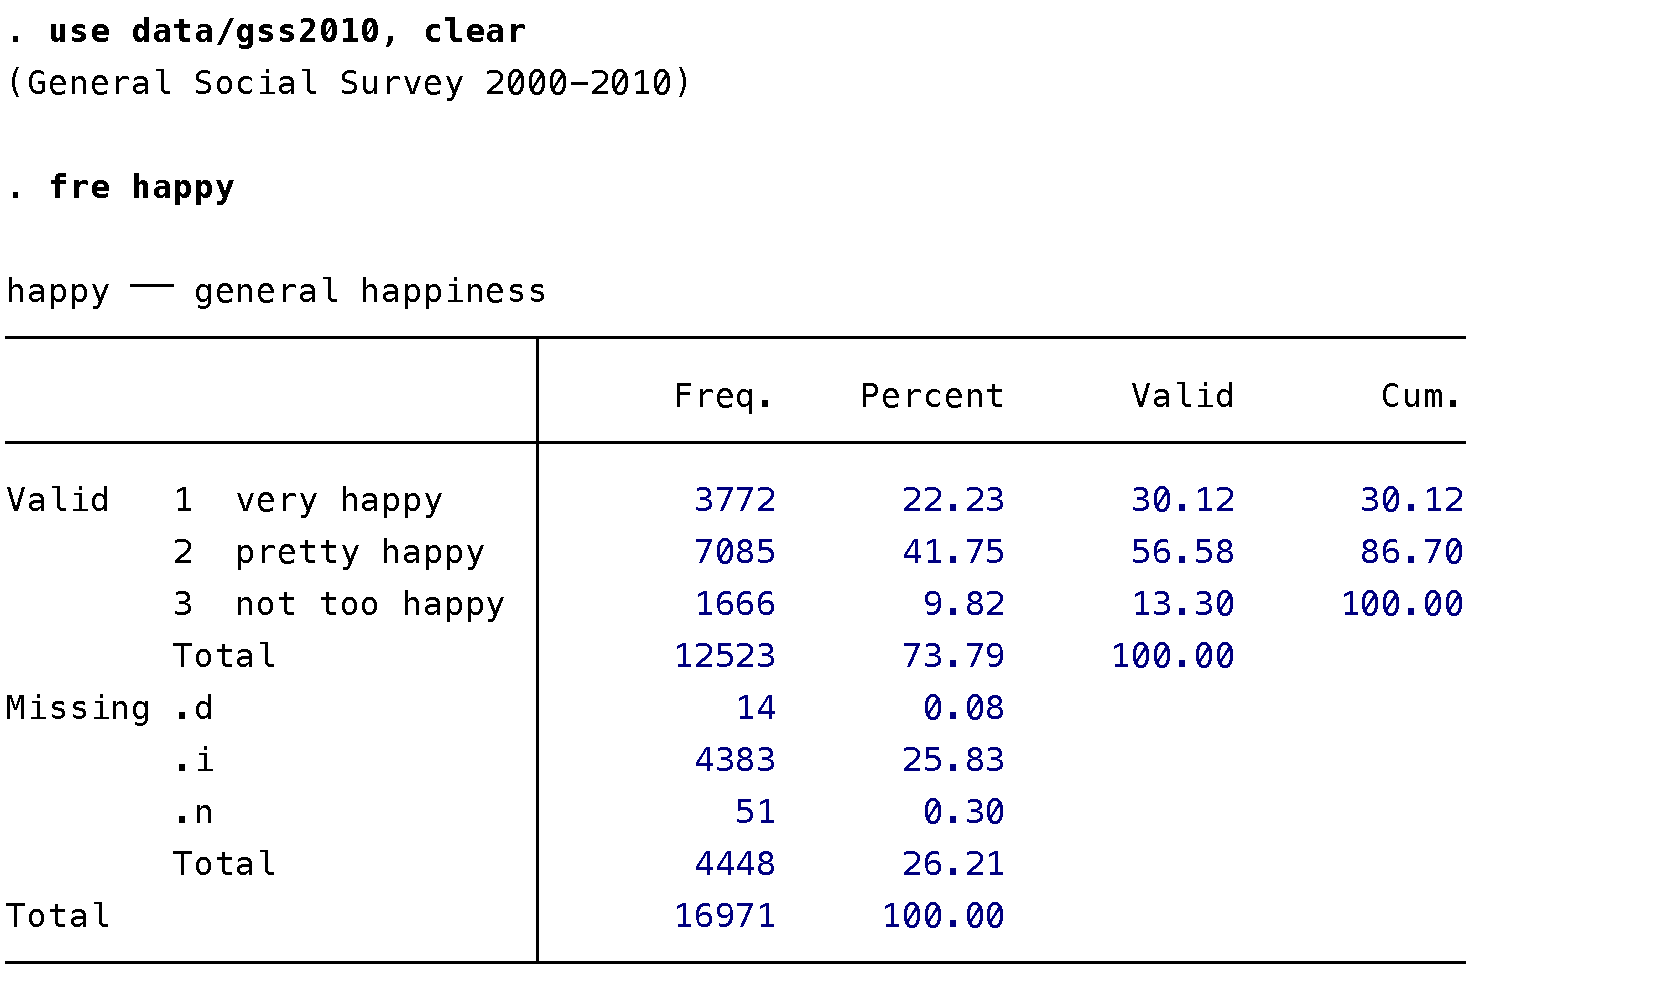
\includegraphics{gss-happiness}

The variable can be easily reversed to the opposite coding by substracting the scale to its maximum $+ 1$, and then by relabelling the values of the new variable:

\begin{fullwidth}
	\begin{docspec}
		gen happiness:happiness = 4 - happy\\
		la def happiness 1 "Not too happy" 2 "Pretty happy" 3 "Very happy", replace\\
		fre happiness
	\end{docspec}
\end{fullwidth}

In the example above, the \cmd[gen]{generate} command handles the numeric reverse by creating a new variable called \texttt{happiness}, for which a \emph{value label} is simultaneously defined under the same name. The label is then defined with the \cmd[la def]{label define} command, so that the new variable will show the same text labels than the original one:\\[1em]

	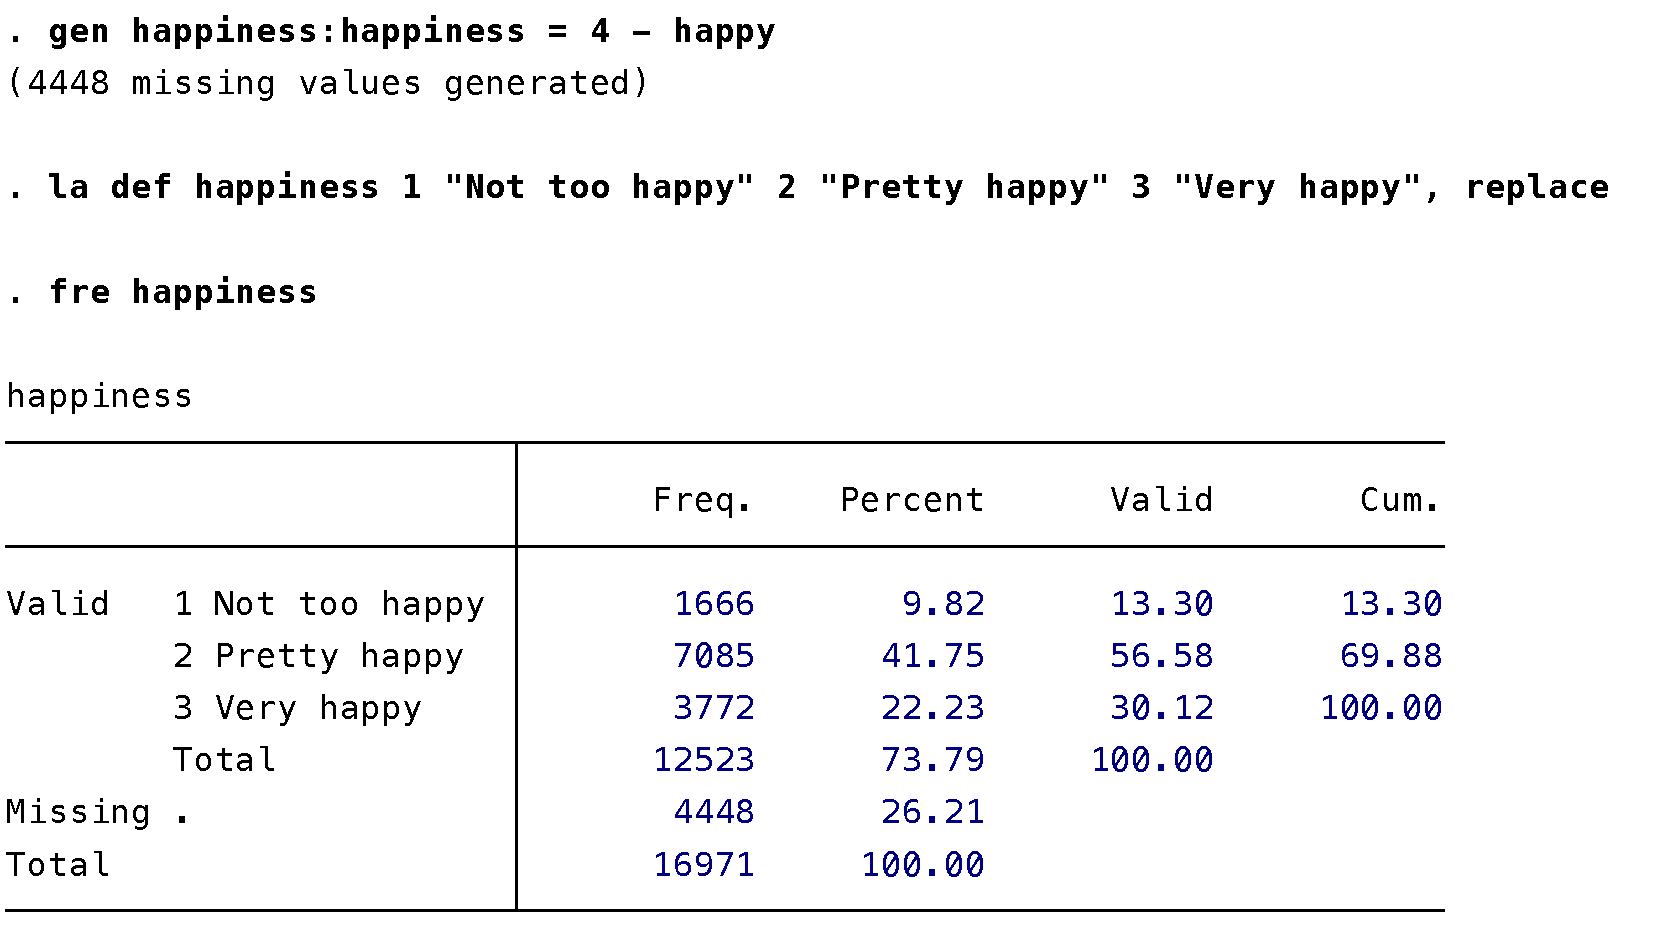
\includegraphics{gss-happiness-reverse-coding}\\[1em]

\index{Labels!For values}%
Stata syntax for value labels is pretty straightforward. The trick is to remember to assign the value label to the variable, or the labels will not show. This can be done through the \texttt{gen x:x} trick shown above, or through the \cmd[la val]{label values} command. One value label can be applied to any number of variables: a generic `yes/no' value label can therefore be applied to several variables at once.%
	\footnote{This system is not only convenient, it is also a way to compress the data.}
Type \texttt{h la} for further illustrations of value labels.

	\item[Recoding to less groups]% % % % % % % % %
	%
Another common situation is having to recode a categorical variable to less groups than it originally had, in order to create groups large enough for cross-tabulation and statistical testing. The next example shows an extract of the \ess, in which left-right positioning has been measured on an 11-point scale coded from 0 (extreme-left) to 11 (extreme-right):

\begin{docspec}
	use data/ess2008 if cntry == "HU", clear\\
	fre lrscale
\end{docspec}

The extract loads only the data for Hungary ($N = 1544$ respondents). We should consider recoding the scale to less precise but more populated categories, because the number of respondents at each level of the scale is often very low and threatens to provide too little statistical power:\\[1em]

	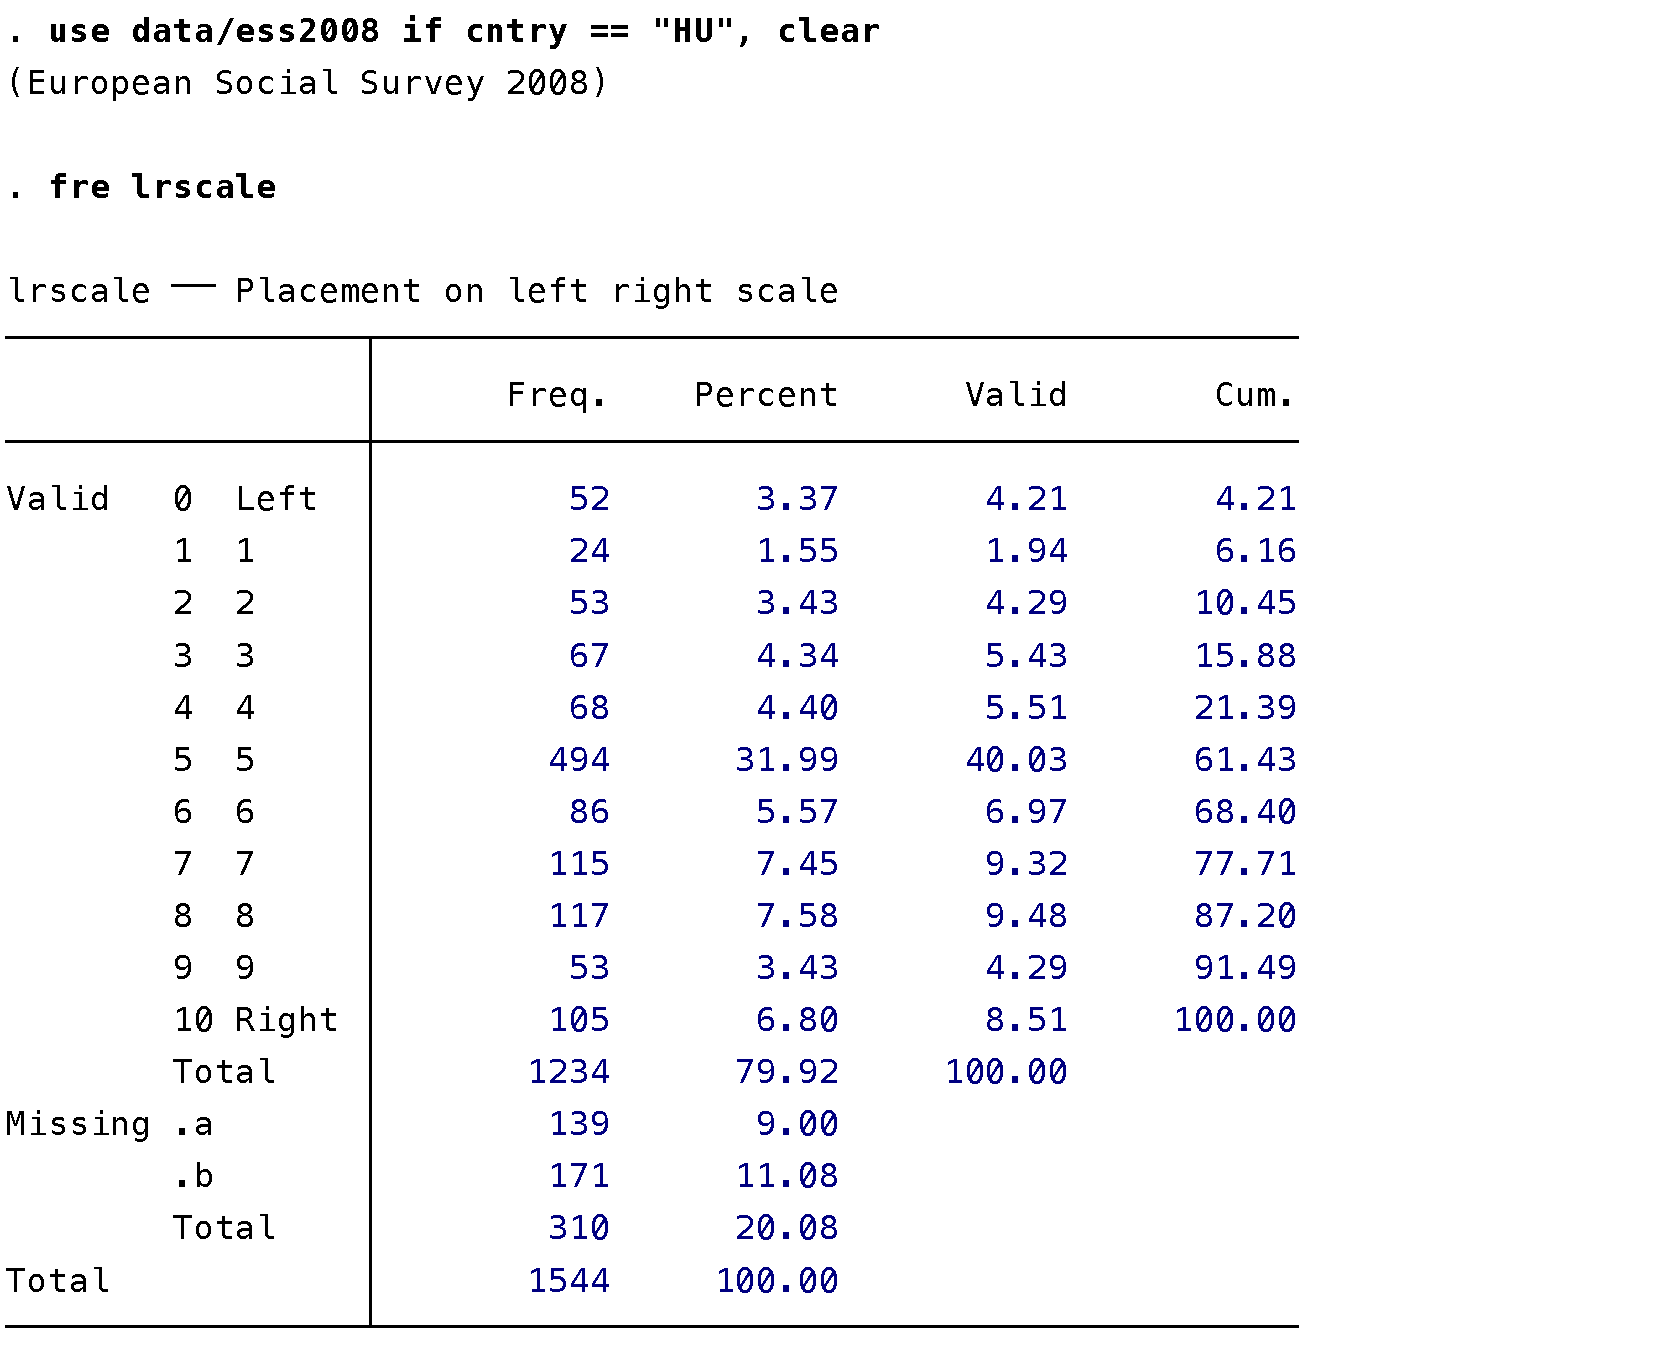
\includegraphics{ess-load-hungary-lrscale}\\[1em]

	\item[Recoding to intervals]% % % % % % % % %
	%

	\item[Recoding to dummies]% % % % % % % % %
	%
A specific case of recoding is when you are recoding to only two values, he female dummy recode from p.~\pageref{female-dummy} we have used a logical statement

	\item[Encoding a string variable]% % % % % % % % %
	%
	% encode
	
	\item[Replacing a string value]% % % % % % % % %
	%
	% replace
	
\end{description}